\documentclass[a4paper,11pt]{book}
%\documentclass[a4paper,twoside,11pt,titlepage]{book}
\usepackage{listings}
\usepackage[utf8]{inputenc}
\usepackage[spanish]{babel}
\usepackage{subcaption}
\usepackage{algorithm}
\usepackage{algpseudocode}

% \usepackage[style=list, number=none]{glossary} %
%\usepackage{titlesec}
%\usepackage{pailatino}
\usepackage{float}

\decimalpoint
\usepackage{dcolumn}
\newcolumntype{.}{D{.}{\esperiod}{-1}}
\makeatletter
\addto\shorthandsspanish{\let\esperiod\es@period@code}
\makeatother

\usepackage{enumitem}
\usepackage{amsmath}
%\usepackage[chapter]{algorithm}
\RequirePackage{verbatim}
%\RequirePackage[Glenn]{fncychap}
\usepackage{fancyhdr}
\usepackage{graphicx}
\usepackage{afterpage}

\usepackage{longtable}

\usepackage[hidelinks]{hyperref}
% ********************************************************************
% Re-usable information
% ********************************************************************
\newcommand{\myTitle}{Implementación optimizada sobre sistemas heterogéneos de algoritmos de Deep Learning para clasificación de imágenes\xspace}
\newcommand{\myDegree}{Grado en Ingeniería Informática\xspace}
\newcommand{\myName}{David Sánchez Pérez \xspace}
\newcommand{\myProf}{José Miguel Mantas Ruiz \xspace}
%\newcommand{\mySupervisor}{Put name here\xspace}
\newcommand{\myFaculty}{Escuela Técnica Superior de Ingenierías Informática y de
Telecomunicación\xspace}
\newcommand{\myFacultyShort}{E.T.S. de Ingenierías Informática y de
Telecomunicación\xspace}
\newcommand{\myDepartment}{Departamento de Lenguajes y Sistemas Informáticos\xspace}
\newcommand{\myUni}{\protect{Universidad de Granada}\xspace}
\newcommand{\myLocation}{Granada\xspace}
\newcommand{\myTime}{\today\xspace}
\newcommand{\myVersion}{Version 0.1\xspace}


\hypersetup{
pdfauthor = {\myName (email (en) ugr (punto) es)},
pdftitle = {\myTitle},
pdfsubject = {},
pdfkeywords = {palabra_clave1, palabra_clave2, palabra_clave3, ...},
pdfcreator = {LaTeX con el paquete ....},
pdfproducer = {pdflatex}
}

%\hyphenation{}


%\usepackage{doxygen/doxygen}
%\usepackage{pdfpages}
\usepackage{url}
\usepackage{colortbl,longtable}
\usepackage[stable]{footmisc}
%\usepackage{index}

%\makeindex
%\usepackage[style=long, cols=2,border=plain,toc=true,number=none]{glossary}
% \makeglossary

% Definición de comandos que me son tiles:
%\renewcommand{\indexname}{Índice alfabético}
%\renewcommand{\glossaryname}{Glosario}

\pagestyle{fancy}
\fancyhf{}
\fancyhead[LO]{\leftmark}
\fancyhead[RE]{\rightmark}
\fancyhead[RO,LE]{\textbf{\thepage}}
\renewcommand{\chaptermark}[1]{\markboth{\textbf{#1}}{}}
\renewcommand{\sectionmark}[1]{\markright{\textbf{\thesection. #1}}}

\setlength{\headheight}{1.5\headheight}

\newcommand{\HRule}{\rule{\linewidth}{0.5mm}}
%Definimos los tipos teorema, ejemplo y definición podremos usar estos tipos
%simplemente poniendo \begin{teorema} \end{teorema} ...
\newtheorem{teorema}{Teorema}[chapter]
\newtheorem{ejemplo}{Ejemplo}[chapter]
\newtheorem{definicion}{Definición}[chapter]

\definecolor{gray97}{gray}{.97}
\definecolor{gray75}{gray}{.75}
\definecolor{gray45}{gray}{.45}
\definecolor{gray30}{gray}{.94}

\lstset{ frame=Ltb,
     framerule=0.5pt,
     aboveskip=0.5cm,
     framextopmargin=3pt,
     framexbottommargin=3pt,
     framexleftmargin=0.1cm,
     framesep=0pt,
     rulesep=.4pt,
     backgroundcolor=\color{gray97},
     rulesepcolor=\color{black},
     %
     stringstyle=\ttfamily,
     showstringspaces = false,
     basicstyle=\scriptsize\ttfamily,
     commentstyle=\color{gray45},
     keywordstyle=\bfseries,
     %
     numbers=left,
     numbersep=6pt,
     numberstyle=\tiny,
     numberfirstline = false,
     breaklines=true,
   }
 
% minimizar fragmentado de listados
\lstnewenvironment{listing}[1][]
   {\lstset{#1}\pagebreak[0]}{\pagebreak[0]}

\lstdefinestyle{CodigoC}
   {
	basicstyle=\scriptsize,
	frame=single,
	language=C,
	numbers=left
   }
\lstdefinestyle{CodigoC++}
   {
	basicstyle=\small,
	frame=single,
	backgroundcolor=\color{gray30},
	language=C++,
	numbers=left
   }

 
\lstdefinestyle{Consola}
   {basicstyle=\scriptsize\bf\ttfamily,
    backgroundcolor=\color{gray30},
    frame=single,
    numbers=none
   }


\newcommand{\bigrule}{\titlerule[0.5mm]}


%Para conseguir que en las páginas en blanco no ponga cabecerass
\makeatletter
\def\clearpage{%
  \ifvmode
    \ifnum \@dbltopnum =\m@ne
      \ifdim \pagetotal <\topskip
        \hbox{}
      \fi
    \fi
  \fi
  \newpage
  \thispagestyle{empty}
  \write\m@ne{}
  \vbox{}
  \penalty -\@Mi
}
\makeatother

\usepackage{pdfpages}
\begin{document}
\begin{titlepage}
 
 
\newlength{\centeroffset}
\setlength{\centeroffset}{-0.5\oddsidemargin}
\addtolength{\centeroffset}{0.5\evensidemargin}
\thispagestyle{empty}

\noindent\hspace*{\centeroffset}\begin{minipage}{\textwidth}

\centering

\includegraphics[width=0.9\textwidth]{imagenes/logo_ugr.jpg}\\[1.4cm]

\textsc{ \Large TRABAJO FIN DE GRADO\\[0.2cm]}
\textsc{ INGENIERÍA EN ...}\\[1cm]
% Upper part of the page
% 
% Title
{\Huge\bfseries Titulo del Proyecto\\
}
\noindent\rule[-1ex]{\textwidth}{3pt}\\[3.5ex]
{\large\bfseries Subtitulo del Proyecto}
\end{minipage}

\vspace{2.5cm}
\noindent\hspace*{\centeroffset}\begin{minipage}{\textwidth}
\centering

\textbf{Autor}\\ {Nombre Apellido1 Apellido2 (alumno)}\\[2.5ex]
\textbf{Directores}\\
{Nombre Apellido1 Apellido2 (tutor1)\\
Nombre Apellido1 Apellido2 (tutor2)}\\[2cm]

\includegraphics[width=0.3\textwidth]{imagenes/etsiit_logo.png}\\[0.1cm]
\textsc{Escuela Técnica Superior de Ingenierías Informática y de Telecomunicación}\\
\textsc{---}\\
Granada, mes de 201
\end{minipage}
%\addtolength{\textwidth}{\centeroffset}
%\vspace{\stretch{2}}
\end{titlepage}



\chapter*{}
%\thispagestyle{empty}
%\cleardoublepage

%\thispagestyle{empty}

\begin{titlepage}
 
 
\setlength{\centeroffset}{-0.5\oddsidemargin}
\addtolength{\centeroffset}{0.5\evensidemargin}
\thispagestyle{empty}

\noindent\hspace*{\centeroffset}\begin{minipage}{\textwidth}

\centering
%
\includegraphics[width=0.9\textwidth]{imagenes/logo_ugr.jpg}\\[1.4cm]

%\textsc{ \Large PROYECTO FIN DE CARRERA\\[0.2cm]}
%\textsc{ INGENIERÍA EN INFORMÁTICA}\\[1cm]
% Upper part of the page
% 

 \vspace{3.3cm}

%si el proyecto tiene logo poner aquí

\includegraphics{imagenes/logo.png} 
 \vspace{0.5cm}

% Title

{\Huge\bfseries Título del proyecto\\
}
\noindent\rule[-1ex]{\textwidth}{3pt}\\[3.5ex]
{\large\bfseries Subtítulo del proyecto.\\[4cm]}
\end{minipage}

\vspace{2.5cm}
\noindent\hspace*{\centeroffset}\begin{minipage}{\textwidth}
\centering

\textbf{Autor}\\ {Nombre Apellido1 Apellido2 (alumno)}\\[2.5ex]
\textbf{Directores}\\
{Nombre Apellido1 Apellido2 (tutor1)\\
Nombre Apellido1 Apellido2 (tutor2)}\\[2cm]
%
\includegraphics[width=0.15\textwidth]{imagenes/tstc.png}\\[0.1cm]
%\textsc{Departamento de Teoría de la Señal, Telemática y Comunicaciones}\\
%\textsc{---}\\
%Granada, mes de 201
\end{minipage}
%\addtolength{\textwidth}{\centeroffset}
\vspace{\stretch{2}}

 
\end{titlepage}






\cleardoublepage
\thispagestyle{empty}

\begin{center}
{\large\bfseries Implementación optimizada sobre sistemas heterogéneos de algoritmos de Deep Learning para clasificación de imágenes}\\
\end{center}
\begin{center}
David Sánchez Pérez\\
\end{center}

%\vspace{0.7cm}
\noindent{\textbf{Palabras clave}: Inteligencia Artificial, Aprendizaje Automático, Aprendizaje Profundo, Arquitectura de Redes Neuronales, Procesamiento de Imágenes, Algoritmos de Aprendizaje Automático, Implementación en C++, Paralelización con OpenMP, Miltihilo, Computación en GPU, Programación CUDA, NVIDIA CUDA, Biblioteca cuDNN, Implementaciones Personalizadas}\\

\vspace{0.7cm}
\noindent{\textbf{Resumen}}\\

Este \textit{Trabajo de Fin de Grado} se centra en la aplicación de la computación heterogénea a bajo nivel para optimizar el rendimiento de redes neuronales convolucionales (CNNs). Las CNNs son esenciales en una variedad de campos, incluyendo el reconocimiento de imágenes, la visión artificial, la detección de objetos y el procesamiento del lenguaje natural. 

El enfoque del proyecto es diseñar y desarrollar diversas implementaciones para optimizar la combinación de CPUs y GPUs en algoritmos de aprendizaje profundo. En primer lugar, se diseñará la arquitectura de las redes neuronales convolucionales a implementar. A continuación, se llevará a cabo una implementación secuencial en CPU, seguida de una implementación paralela en CPU utilizando OpenMP. Posteriormente, se desarrollará un sistema heterogéneo empleando CUDA, y, finalmente, se implementará otro sistema heterogéneo utilizando la biblioteca cuDNN.

Cada implementación será construida desde cero, sin depender de bibliotecas o frameworks externos, salvo por OpenMP, CUDA y cuDNN, con el objetivo de consolidar los conocimientos sobre CNNs y su optimización en sistemas heterogéneos.
\cleardoublepage


\thispagestyle{empty}


\begin{center}
{\large\bfseries Optimized Implementation of Deep Learning Algorithms for Image Classification on Heterogeneous Systems}\\
\end{center}
\begin{center}
David Sánchez Pérez\\
\end{center}

%\vspace{0.7cm}
\noindent{\textbf{Keywords}: Artificial Intelligence, Machine Learning, Deep Learning, Computer Vision, Neural Network Architecture, Image Processing, Machine Learning Algorithms, C++ Implementation, OpenMP Parallelization, Miltithreading, GPU Computing, CUDA Programming, NVIDIA CUDA, cuDNN Library, Custom Implementations}\\

\vspace{0.7cm}
\noindent{\textbf{Abstract}}\\

This \textit{Bachelor's Thesis} focuses on the application of low-level heterogeneous computing to optimize the performance of convolutional neural networks (CNNs). CNNs are crucial in various fields, including image recognition, computer vision, object detection, and natural language processing.

The project's approach is to design and develop several implementations to enhance the synergy between CPUs and GPUs in deep learning algorithms. First, the architecture of the convolutional neural networks to be implemented will be designed. Next, a sequential implementation on CPU will be carried out, followed by a parallel CPU implementation using OpenMP. Subsequently, a heterogeneous system using CUDA will be developed, and finally, another heterogeneous system utilizing the cuDNN library will be implemented.

Each implementation will be built from scratch, without relying on external libraries or frameworks, except for OpenMP, CUDA, and cuDNN, with the aim of consolidating knowledge about CNNs and their optimization on heterogeneous systems.

\chapter*{}
\thispagestyle{empty}

\noindent\rule[-1ex]{\textwidth}{2pt}\\[4.5ex]

Yo, \textbf{Nombre Apellido1 Apellido2}, alumno de la titulación TITULACIÓN de la \textbf{Escuela Técnica Superior
de Ingenierías Informática y de Telecomunicación de la Universidad de Granada}, con DNI XXXXXXXXX, autorizo la
ubicación de la siguiente copia de mi Trabajo Fin de Grado en la biblioteca del centro para que pueda ser
consultada por las personas que lo deseen.

\vspace{6cm}

\noindent Fdo: Nombre Apellido1 Apellido2

\vspace{2cm}

\begin{flushright}
Granada a X de mes de 201 .
\end{flushright}


\chapter*{}
\thispagestyle{empty}

\noindent\rule[-1ex]{\textwidth}{2pt}\\[4.5ex]

D. \textbf{Nombre Apellido1 Apellido2 (tutor1)}, Profesor del Área de XXXX del Departamento YYYY de la Universidad de Granada.

\vspace{0.5cm}

D. \textbf{Nombre Apellido1 Apellido2 (tutor2)}, Profesor del Área de XXXX del Departamento YYYY de la Universidad de Granada.


\vspace{0.5cm}

\textbf{Informan:}

\vspace{0.5cm}

Que el presente trabajo, titulado \textit{\textbf{Título del proyecto, Subtítulo del proyecto}},
ha sido realizado bajo su supervisión por \textbf{Nombre Apellido1 Apellido2 (alumno)}, y autorizamos la defensa de dicho trabajo ante el tribunal
que corresponda.

\vspace{0.5cm}

Y para que conste, expiden y firman el presente informe en Granada a X de mes de 201 .

\vspace{1cm}

\textbf{Los directores:}

\vspace{5cm}

\noindent \textbf{Nombre Apellido1 Apellido2 (tutor1) \ \ \ \ \ Nombre Apellido1 Apellido2 (tutor2)}

\chapter*{Agradecimientos}
\thispagestyle{empty}

       \vspace{1cm}


Poner aquí agradecimientos...


\frontmatter
\tableofcontents
\listoffigures
\listoftables
%
\mainmatter
%\setlength{\parskip}{5pt}

\input{capitulos/01\_Introduccion}
\input{capitulos/02\_Conceptos_Previos}
\input{capitulos/04\_Adaptacion\_GPU}
\input{capitulos/05\_Plataformas}
\input{capitulos/06\_Conclusiones}

\appendix

\chapter{cuDNN, Principales funciones} \label{apendice_cuDNN_principales_funciones}

A continuación se mencionarán las principales funciones de cuDNN que se han empleado en este proyecto, siendo las responsables tanto de la propagación hacia delante como de la retropropagación en capas convolucionales y de agrupación máxima, entre otras.

\subsubsection{cudnnConvolutionForward} \label{cudnnConvolutionForward}
Realiza la propagación hacia delante en una capa convolucional.

\begin{verbatim}
	cudnnStatus_t cudnnConvolutionForward(
	cudnnHandle_t                       handle,
	const void                         *alpha,
	const cudnnTensorDescriptor_t       xDesc,
	const void                         *x,
	const cudnnFilterDescriptor_t       wDesc,
	const void                         *w,
	const cudnnConvolutionDescriptor_t  convDesc,
	cudnnConvolutionFwdAlgo_t           algo,
	void                               *workSpace,
	size_t                              workSpaceSizeInBytes,
	const void                         *beta,
	const cudnnTensorDescriptor_t       yDesc,
	void                               *y)
\end{verbatim}

\begin{enumerate}
	\item \textbf{handle}: Manejador.
	\item \textbf{alpha, beta}: Punteros a escalares empleados para combinar los resultados con valores anteriores tal que valor\_final = alpha*result + beta*valor\_anterior.
	\item \textbf{xDesc}: Descriptor asociado al tensor de entrada.
	\item \textbf{x}: Puntero a los datos de entrada en GPU asociados con el descriptor de tensor xDesc.
	\item \textbf{wDesc}: Descriptor asociado al tensor de pesos.
	\item \textbf{w}: Puntero a los pesos en GPU asociados con el descriptor de tensor wDesc.
	\item \textbf{convDesc}: Descriptor de convolución.
	\item \textbf{algo}: Especifica qué algoritmo de convolución aplicar.
	\item \textbf{workSpace}: Puntero a un espacio de trabajo en memoria de GPU.
	\item \textbf{workSpaceSizeInBytes}: Especifica el tamaño en bytes de workSpace.
	\item \textbf{yDesc}: Descriptor asociado al tensor de salida.
	\item \textbf{y}: Puntero a los datos de salida en GPU asociados con el descriptor de tensor yDesc.
\end{enumerate}
\cite{cuDNN_conv_fwd}

\subsubsection{cudnnPoolingForward} \label{cudnnPoolingForward}
Se encarga de la propagación hacia delante en una capa de agrupación máxima.

\begin{verbatim}
	cudnnStatus_t cudnnPoolingForward(
	cudnnHandle_t                    handle,
	const cudnnPoolingDescriptor_t   poolingDesc,
	const void                      *alpha,
	const cudnnTensorDescriptor_t    xDesc,
	const void                      *x,
	const void                      *beta,
	const cudnnTensorDescriptor_t    yDesc,
	void                            *y)
\end{verbatim}

\begin{enumerate}
	\item \textbf{handle}: Manejador.
	\item \textbf{poolingDesc}: Descriptor de la operación de agrupación.
	\item \textbf{alpha, beta}: Punteros a escalares empleados para combinar los resultados con valores anteriores tal que valor\_final = alpha*result + beta*valor\_anterior.
	\item \textbf{xDesc}: Descriptor asociado al tensor de entrada.
	\item \textbf{x}: Puntero a los datos de entrada en GPU asociados con el descriptor de tensor xDesc.
	\item \textbf{yDesc}: Descriptor asociado al tensor de salida.
	\item \textbf{y}: Puntero a los datos de salida en GPU asociados con el descriptor de tensor yDesc.
\end{enumerate}
\cite{cuDNN_pool_fwd}

\subsubsection{cudnnPoolingBackward} \label{cudnnPoolingBackward}
Realiza la retropropagación en una capa de agrupación máxima.

\begin{verbatim}
	cudnnStatus_t cudnnPoolingBackward(
	cudnnHandle_t                       handle,
	const cudnnPoolingDescriptor_t      poolingDesc,
	const void                         *alpha,
	const cudnnTensorDescriptor_t       yDesc,
	const void                         *y,
	const cudnnTensorDescriptor_t       dyDesc,
	const void                         *dy,
	const cudnnTensorDescriptor_t       xDesc,
	const void                         *xData,
	const void                         *beta,
	const cudnnTensorDescriptor_t       dxDesc,
	void                               *dx)
\end{verbatim}

\begin{enumerate}
	\item \textbf{handle}: Manejador.
	\item \textbf{poolingDesc}: Descriptor de la operación de agrupación.
	\item \textbf{alpha, beta}: Punteros a escalares empleados para combinar los resultados con valores anteriores tal que valor\_final = alpha*result + beta*valor\_anterior.
	\item \textbf{yDesc}: Descriptor asociado al tensor de salida.
	\item \textbf{y}: Puntero a los datos de salida en GPU asociados con el descriptor de tensor yDesc.
	\item \textbf{dyDesc}: Descriptor asociado al tensor que almacena el gradiente de la pérdida respecto a los datos de salida.
	\item \textbf{dy}: Puntero al gradiente de la pérdida respecto a los datos de salida en GPU asociados con el descriptor de tensor dyDesc.
	\item \textbf{xDesc}: Descriptor asociado al tensor de entrada.
	\item \textbf{x}: Puntero a los datos de entrada en GPU asociados con el descriptor de tensor xDesc.
	\item \textbf{dxDesc}: Descriptor asociado al tensor que almacena el gradiente de la pérdida respecto a los datos de entrada.
	\item \textbf{dx}: Puntero al gradiente de la pérdida respecto a los datos de entrada en GPU asociados con el descriptor de tensor dxDesc.	
\end{enumerate}
\cite{cuDNN_pool_fwd}

\subsubsection{cudnnConvolutionBackwardFilter} \label{cudnnConvolutionBackwardFilter}
Realiza la retropropagación respecto a los pesos en una capa convolucional.

\begin{verbatim}
	cudnnStatus_t cudnnConvolutionBackwardFilter(
	cudnnHandle_t                       handle,
	const void                         *alpha,
	const cudnnTensorDescriptor_t       xDesc,
	const void                         *x,
	const cudnnTensorDescriptor_t       dyDesc,
	const void                         *dy,
	const cudnnConvolutionDescriptor_t  convDesc,
	cudnnConvolutionBwdFilterAlgo_t     algo,
	void                               *workSpace,
	size_t                              workSpaceSizeInBytes,
	const void                         *beta,
	const cudnnFilterDescriptor_t       dwDesc,
	void                               *dw)
\end{verbatim}

\begin{enumerate}
	\item \textbf{handle}: Manejador.
	\item \textbf{alpha, beta}: Punteros a escalares empleados para combinar los resultados con valores anteriores tal que valor\_final = alpha*result + beta*valor\_anterior.
	\item \textbf{xDesc}: Descriptor asociado al tensor de entrada.
	\item \textbf{x}: Puntero a los datos de entrada en GPU asociados con el descriptor de tensor xDesc.	
	\item \textbf{dyDesc}: Descriptor asociado al tensor que almacena el gradiente de la pérdida respecto a los datos de salida.
	\item \textbf{dy}: Puntero al gradiente de la pérdida respecto a los datos de salida en GPU asociados con el descriptor de tensor dyDesc.
	\item \textbf{convDesc}: Descriptor de convolución.
	\item \textbf{algo}: Especifica qué algoritmo de convolución aplicar.
	\item \textbf{workSpace}: Puntero a un espacio de trabajo en memoria de GPU.
	\item \textbf{workSpaceSizeInBytes}: Especifica el tamaño en bytes de workSpace.
	\item \textbf{dwDesc}: Descriptor del tensor asociado al gradiente de la pérdida respecto a los pesos.
	\item \textbf{dw}: Puntero al gradiente de los pesos en GPU asociados con el descriptor de tensor dwDesc.
\end{enumerate}
\cite{cuDNN_conv_back_w}


\subsubsection{cudnnConvolutionBackwardData} \label{cudnnConvolutionBackwardData}
Realiza la retropropagación respecto a los datos de entrada en una capa convolucional.

\begin{verbatim}
	cudnnStatus_t cudnnConvolutionBackwardData(
	cudnnHandle_t                       handle,
	const void                         *alpha,
	const cudnnFilterDescriptor_t       wDesc,
	const void                         *w,
	const cudnnTensorDescriptor_t       dyDesc,
	const void                         *dy,
	const cudnnConvolutionDescriptor_t  convDesc,
	cudnnConvolutionBwdDataAlgo_t       algo,
	void                               *workSpace,
	size_t                              workSpaceSizeInBytes,
	const void                         *beta,
	const cudnnTensorDescriptor_t       dxDesc,
	void                               *dx)
\end{verbatim}

\begin{enumerate}
	\item \textbf{handle}: Manejador.
	\item \textbf{alpha, beta}: Punteros a escalares empleados para combinar los resultados con valores anteriores tal que valor\_final = alpha*result + beta*valor\_anterior.
	\item \textbf{wDesc}: Descriptor asociado al tensor de pesos.
	\item \textbf{w}: Puntero a los pesos en GPU asociados con el descriptor de tensor wDesc.
	\item \textbf{dyDesc}: Descriptor asociado al tensor que almacena el gradiente de la pérdida respecto a los datos de salida.
	\item \textbf{dy}: Puntero al gradiente de la pérdida respecto a los datos de salida en GPU asociados con el descriptor de tensor dyDesc.
	\item \textbf{convDesc}: Descriptor de convolución.
	\item \textbf{algo}: Especifica qué algoritmo de convolución aplicar.
	\item \textbf{workSpace}: Puntero a un espacio de trabajo en memoria de GPU.
	\item \textbf{workSpaceSizeInBytes}: Especifica el tamaño en bytes de workSpace.
	\item \textbf{dxDesc}: Descriptor asociado al tensor que almacena el gradiente de la pérdida respecto a los datos de entrada.
	\item \textbf{dx}: Puntero al gradiente de la pérdida respecto a los datos de entrada en GPU asociados con el descriptor de tensor dxDesc.	
\end{enumerate}
\cite{cuDNN_conv_back_x}


\chapter{Planificación detallada} \label{planificacion}

Para el desarrollo de este proyecto, se ha requerido llevar a cabo una serie de tareas con diferentes dificultades e importancias. A continuación, se muestra una planificación general del mismo en la tabla \ref{tabla_planificación_aprendice}, junto con las fases que componen su desarrollo, y una planificación temporal de cada apartado por separado. Cabe destacar que, cada apartado, se basa en los conocimientos adquiridos en los apartados anteriores, a la vez que introduce conceptos nuevos y mejora las prestaciones del modelo. De esta manera, cada apartado supondrá retos nuevos nunca antes vistos y, si un apartado anterior presenta algún fallo desconocido en el momento, se deberá volver a la etapa anterior y arreglarlo. Tras solventarlo, se podrá proseguir con la etapa posterior. Además, dada la naturaleza de `caja oscura' de las redes neuronales, estas presentan cierta dificultad a la hora de depurar el código. Por tanto, esto supondrá un tiempo de depuración considerable en todas y cada una de las implementaciones, tal y como se mostrará a continuación.

\begin{enumerate}[label=\textbullet]
	\item \textbf{Estudio previo}: Consiste en el estudio y comprensión de cuestiones generales, dentro del campo de aprendizaje automático y visión por computador, comunes a redes neuronales totalmente conectadas, y redes neuronales convolucionales.
	\begin{enumerate}[label=\textbullet]
		\item Investigación, comprensión y selección de funciones de activación a emplear (4 horas)
		\item Investigación y comprensión sobre el algoritmo del descenso del gradiente (3 horas)
		\item Investigación y comprensión sobre el entrenamiento una red neuronal (2 horas)
		\item Investigación y comprensión de sistemas heterogéneos y sistemas homogéneos (3 horas)
		\item Investigación y comprensión de sistemas heterogéneos aplicados a CNNs (4 horas)
	\end{enumerate}
	
	\item \textbf{Investigación y desarrollo de redes neuronales totalmente conectadas}: En este periodo, me centré en la investigación y comprensión sobre las redes neuronales totalmente conectadas a bajo nivel. De esta manera, sabía que podría generar cualquier tipo de red totalmente conectada de manera dinámica, sin necesidad de realizar ningún tipo de cálculo posterior, independientemente del lenguaje de programación empleado, así como del uso o no de librerías que faciliten el proceso. 
	\begin{enumerate}[label=\textbullet]
		\item Investigación y desarrollo teórico de la retropropagación en una red totalmente conectada con 1 capa oculta (40 horas)
		\item Investigación y desarrollo teórico de la retropropagación en una red totalmente conectada con 2 capas ocultas (9 horas)
		\item Desarrollo teórico de la retropropagación en una red totalmente conectada con N capas ocultas (5 horas)
		\item Investigación y desarrollo teórico sobre la retropropagación en una capa SoftMax (7 horas)
		\item Implementación en C++ sobre la retropropagación en una capa softmax (8 horas)
		\item Investigación y desarrollo del algoritmo del descenso del gradiente en una red totalmente conectada en C++ (2 horas)
		\item Investigación sobre distintas inicializaciones de pesos e implementación de la inicialización de pesos HE (2 horas)	
		\item Realización de pruebas prácticas de funcionamiento con distintas bases de datos y arquitecturas de modelos (10 horas)	
		\item Implementación en C++ sobre cuestiones generales de una red neuronal totalmente conectada como entrenamiento, lectura de imágenes, creación, gestión y actualización de pesos y sesgos, evaluación del modelo sobre un conjunto de datos, creación de estructura general, etc (60 horas).
	\end{enumerate}
	\item \textbf{Investigación y desarrollo de redes neuronales convolucionales}:
	Una vez familiarizado con redes neuronales totalmente conectadas, se trató de comprender de igual forma las redes neuronales convolucionales, pues se encuentran ampliamente relacionadas.
	\begin{enumerate}[label=\textbullet]
		\item Investigación y desarrollo teórico de la propagación hacia delante en una capa convolucional de una red neuronal convolucional (5 horas)
		\item Investigación y desarrollo teórico de la retropropagación en una capa convolucional con y sin relleno en una red neuronal convolucional (21 horas)
		\item Investigación y desarrollo teórico sobre el relleno en una red neuronal convolucional (12 horas)
		\item Desarrollo de conclusiones teóricas con respecto a retropropagación en capa convolucional con y sin relleno (4 horas)
		\item Investigación y desarrollo teórico sobre una capa de agrupación máxima en una red neuronal convolucional (8 horas)
		\item Investigación y desarrollo teórico sobre una capa de aplanado en una red neuronal convolucional (1 hora)
		\item Implementación en C++ sobre la propagación hacia delante en una capa convolucional de una red neuronal convolucional (8 horas).
		\item Implementación en C++ sobre la retropropagación en una capa convolucional de una red neuronal convolucional (12 horas).
		\item Implementación en C++ sobre la propagación hacia delante en una capa de agrupación máxima de una red neuronal convolucional (4 horas).
		\item Implementación en C++ sobre la retropropagación en una capa de agrupación máxima de una red neuronal convolucional (6 horas).
		\item Implementación en C++ sobre una capa de aplanado de una red neuronal convolucional (1 hora).
		\item Implementación en C++ sobre cuestiones generales de una CNN como entrenamiento, lectura de imágenes, evaluación del modelo sobre un conjunto de datos, creación de estructura general, etc (70 horas).
	\end{enumerate}
	\item \textbf{Investigación y desarrollo de sistemas homogéneos con OpenMP}:
	Una vez, comprendido el funcionamiento tanto de las redes neuronales totalmente conectadas, como de las redes neuronales convolucionales, me centré en reducir los tiempos de cómputo requeridos en ellas, mediante un paralelismo orientado a datos con OpenMP, (se analizará en detalle en secciones posteriores).
	\begin{enumerate}[label=\textbullet]
		\item Investigación sobre tipos de paralelismo con OpenMP orientados tanto a redes neuronales totalmente conectadas como a redes neuronales convolucionales (4 horas)
		\item Investigación y desarrollo teórico sobre paralelismo a nivel de datos con OpenMP en el algoritmo del descenso del gradiente (3 horas).
		\item Implementación en C++ y OpenMP sobre el algoritmo del descenso del gradiente en la red neuronal totalmente conectada (10 horas).
		\item Implementación en C++ y OpenMP sobre el algoritmo del descenso del gradiente en la red neuronal convolucional (30 horas).
		\item Implementación en C++ y OpenMP sobre aspectos generales de una red neuronal totalmente conectada (20 horas).
		\item Implementación en C++ y OpenMP sobre cuestiones generales de una red neuronal convolucional (30 horas).
		\item Realización de pruebas finales para verificar un correcto entrenamiento y aprendizaje (6 horas)
	\end{enumerate}
	\item \textbf{Investigación y desarrollo de sistemas heterogéneos con CUDA y cuDNN}:
	Con el conocimiento teórico y práctico ya adquirido sobre sistemas homogéneos, aplicados tanto a redes neuronales totalmente conectadas como a redes neuronales convolucionales, se avanza ahora hacia la exploración de sistemas heterogéneos, aplicados a estas mismas arquitecturas de redes neuronales.
	\begin{enumerate}[label=\textbullet]
		\item Investigación y desarrollo teórico sobre la propagación hacia delante y retropropagación en una capa convolucional como GEMM (8 horas)
		\item Investigación y desarrollo teórico sobre la propagación hacia delante y retropropagación en una capa de agrupación máxima con CUDA (5 horas)
		\item Investigación y comprensión de la librería cuBLAS (5 horas)
		\item Implementación en C++ sobre la propagación hacia delante en una capa convolucional como GEMM con cuBLAS (6 horas)
		\item Implementación en C++ sobre la retropropagación en una capa convolucional como GEMM con cuBLAS (26 horas)
		\item Investigación y desarrollo teórico y práctico sobre el algoritmo de multiplicación matricial con CUDA empleado (30 horas)
		\item Implementación en C++ y CUDA sobre la capa de agrupación máxima con CUDA (14 horas)
		\item Investigación y desarrollo teórico y práctico sobre la capa totalmente conectada como GEMM (31 horas)
		\item Investigación y desarrollo teórico sobre el consumo de memoria con GEMM (5 horas)
		\item Implementación de aspectos generales de una red neuronal convolucional con CUDA (71 horas).
		\item Sustitución de la clase Vector de la STL en todo el proyecto por punteros necesarios para emplear CUDA (30 horas).
		\item Investigación teórica y adaptación práctica de la implementación con CUDA a cuDNN (51 horas).
	\end{enumerate}
	
\end{enumerate}


\begin{table}[H]
	\centering
	\begin{tabular}{|lll|}
		\hline
		Apartado 	 &\vline  & Tiempo (Horas) \\
		\hline
		
		Estudio previo    & \vline & 16 \\			
		\hline
		Investigación y desarrollo  	 & \vline & 	\\
		de redes neuronales  	 & \vline & 143	\\
		totalmente conectadas 	 & \vline & 	\\
		\hline
		Investigación y desarrollo    & \vline & 	 \\	
		de redes neuronales    & \vline & 152	 \\			
		convolucionales    & \vline & 	 \\					
		\hline
		Investigación y desarrollo  	 & \vline & 	 \\
		de sistemas homogéneos  	 & \vline & 103	 \\
		con OpenMP 	 & \vline & 	 \\
		\hline
		Investigación y desarrollo     & \vline &  	\\
		de sistemas heterogéneos    & \vline &  \\ 
		con CUDA y cuDNN    & \vline & 282 \\ 	
		\hline
		\hline
		Tiempo total:				& \vline & 696 \\
		\hline
	\end{tabular}
	\caption{Planificación del proyecto}
	\label{tabla_planificación_aprendice}
\end{table}

\chapter{Retropropagación en capa SoftMax} \label{softmax_apendice}


Tal y como se comentó en secciones anteriores, se empleará SoftMax en la última capa totalmente conectada. De este modo, se definen los valores de entrada a la misma como \textit{Z}, y los de salida como \textit{O}, tal y como se muestra en la Figura \ref{cross_entropy_notacion_apendice}.

\begin{figure}[H]
	\centering
	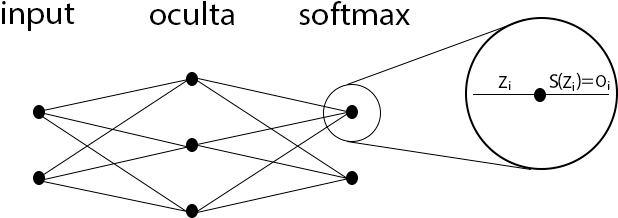
\includegraphics[scale=0.4]{imagenes/NN_softmax.jpg}  
	\caption{Estructura de una red totalmente conectada con softmax en la última capa}
\end{figure}

\begin{gather}
	E = - \sum_{i=1}^{N}  [y_i   ln(O_i)] 
	\label{cross_entropy_notacion_apendice}
\end{gather}

Según esta notación, la función de error \ref{fig:loss_func_softmax} se convierte en la fórmula \ref{cross_entropy_notacion_apendice}.

\section{Cálculo del gradiente de la función de error}

Para comenzar la retropropagación, empezaremos por calcular el gradiente de la función de pérdida con respecto a cada parámetro de entrada de la capa en la cual se aplicó SoftMax, esto se muestra en la fórmula \ref{grad_H_Z}.
\begin{gather}
	\frac{\partial E}{\partial Z_k} = \frac{\partial(- \sum_{i=1}^{H}  [y_i   ln(O_i)])}{\partial Z_k} = - \sum_{i=1}^{H}  [\frac{\partial(y_i   ln(O_i))}{\partial Z_k}] 
	\label{grad_H_Z}
\end{gather}

Como $y_i$ (etiqueta real), es independiente con respecto a $Z_k$ (neurona artificial de entrada), en la fórmula \ref{grad_H_Z}, esta se trata como una constante. \\
\begin{gather}
	\frac{\partial E}{\partial Z_k} = - \sum_{i=1}^{H}  [y_i   \frac{\partial(ln(O_i))}{\partial Z_k}] \notag
\end{gather}

Por simplificar los cálculos y eliminar el logaritmo de la ecuación, se aplica la regla de la cadena, y, como resultado, se obtienen las fórmulas \ref{gradiente_Oi_Zk_1} y \ref{gradiente_Oi_Zk_2}.
\begin{gather}	
	\frac{\partial E}{\partial Z_k} = - \sum_{i=1}^{H}  [y_i   \frac{\partial(ln(O_i))}{\partial O_i}   \frac{\partial O_i}{\partial Z_k}]
	\label{gradiente_Oi_Zk_1} \\
	\frac{\partial E}{\partial Z_k} = - \sum_{i=1}^{H}  [\frac{y_i}{O_i}   \frac{\partial O_i}{\partial Z_k}] 
	\label{gradiente_Oi_Zk_2}
\end{gather}

% ver https://www.mldawn.com/the-derivative-of-softmaxz-function-w-r-t-z/

\section{Derivada de softmax con respecto a su entrada, $\frac{\partial O_i}{\partial Z_k}$}

Una vez obtenida la fórmula \ref{gradiente_Oi_Zk_2}, nos disponemos a calcular la derivada de $O_i$ con respecto $Z_i$. \\
Sin embargo, hay que contemplar 2 casos posibles, siendo estos $\frac{\partial S(Z_i)}{\partial Z_i}$ y $\frac{\partial S(Z_i)}{\partial Z_j}$, donde i $\neq$ j. \\

\section{Caso $\frac{\partial S(Z_i)}{\partial Z_i}$}

\begin{gather}
	\frac{\partial f(x)}{\partial g(x)} = \frac{f'(x) g(x) - g'(x) f(x)}{g(x)^2} \\
	S(z_i) = \frac{e^{Z_i}}{e^{Z_1} + ... + e^{Z_H}} \notag \\
	\frac{\partial S(Z_1)}{\partial Z_1} = \frac{[\frac{\partial e^{Z_1}}{\partial Z_1}   (e^{Z_1} + ... + e^{Z_H}) ] - [\frac{\partial (e^{Z_1} + ... + e^{Z_H})}{\partial Z_1}   e^{Z_1} ] }{(e^{Z_1} + ... + e^{Z_H})^2} \notag
\end{gather}

Se aplica $\frac{\partial e^{Z_1}}{\partial Z_1} = e^{Z_1}$ \\
\begin{gather}
	\frac{\partial S(Z_1)}{\partial Z_1} = \frac{[e^{Z_1}   \sum_{i=1}^{H}  e^{Z_i}] - [e^{Z_1}   e^{Z_1}]   }{ (\sum_{i=1}^{H}  e^{Z_i})^2} \notag \\
\end{gather}

Se saca factor común $e^{Z_1}$ \\
\begin{gather}
	\frac{\partial S(Z_1)}{\partial Z_1} = \frac{e^{Z_1} ([\sum_{i=1}^{H}  e^{Z_i}] - e^{Z_1})  }{(\sum_{i=1}^{H}  e^{Z_i})^2} \notag \\
	\frac{\partial S(Z_1)}{\partial Z_1} = \frac{e^{Z_1}}{\sum_{i=1}^{H}  e^{Z_i}}   \frac{[\sum_{i=1}^{H}  e^{Z_i}] - e^{Z_1}}{\sum_{i=1}^{H}  e^{Z_i}} \notag
\end{gather}

Se recuerda que $\frac{\sum_{i=1}^{H}  e^{Z_i}}{\sum_{i=1}^{H}  e^{Z_i}} = 1$ y que S($Z_1$) = $ \frac{e^{Z_1}}{\sum_{i=1}^{H}  e^{Z_i}}$ \\
\begin{gather}
	\frac{\partial S(Z_1)}{\partial Z_1} = S(Z_1)   (1- S(Z_1))
	\label{grad_Oi_Zk_drch}
\end{gather}

\subsection{Caso $\frac{\partial S(Z_i)}{\partial Z_j}$, con i $\neq$ j}

\begin{gather}
	\frac{\partial S(Z_2)}{\partial Z_1} = \frac{[\frac{\partial e^{Z_2}}{\partial Z_1}   (e^{Z_1} + ... + e^{Z_H}) ] - [\frac{\partial (e^{Z_1} + ... + e^{Z_H})}{\partial Z_1}   e^{Z_2} ] }{(e^{Z_1} + ... + e^{Z_H})^2} \notag \\
	\frac{\partial S(Z_2)}{\partial Z_1} = \frac{[0   [\sum_{i=1}^{H}  e^{Z_i}]] - [e^{Z_1}   e^{Z_2}]   }{ (\sum_{i=1}^{H}  e^{Z_i})^2} \notag \\
	\frac{\partial S(Z_2)}{\partial Z_1} = \frac{-e^{Z_1}   e^{Z_2}  }{(\sum_{i=1}^{H}  e^{Z_i})^2} \notag \\
	\frac{\partial S(Z_2)}{\partial Z_1} = \frac{-e^{Z_1}}{\sum_{i=1}^{H}  e^{Z_i}}   \frac{e^{Z_2}}{\sum_{i=1}^{H}  e^{Z_i}} \notag \\
	\frac{\partial S(Z_2)}{\partial Z_1} = -S(Z_1)   S(Z_2)
	\label{grad_Oi_Zk_izq}
\end{gather}

\section{Combinación de casos}

De esta forma, tendremos que dividir  el proceso en 2 partes, cuando i sea igual a j, y cuando i $\neq$ j. \\
Como todos los casos menos uno pertenecen al caso i $\neq$ k, en la fórmula \ref{comb_casos} se aprecia como la ``parte izquierda'' hace referencia al caso i!=k, mientras que la ``parte derecha'' a i=k. \\
Retomamos la fórmula \ref{gradiente_Oi_Zk_2}, aplicando \ref{grad_Oi_Zk_izq} en la parte izquierda, y \ref{grad_Oi_Zk_drch} en la derecha. \\
\begin{gather}
	\frac{\partial E}{\partial Z_k} = - [\sum_{i!=k}^{H} [\frac{y_i}{O_i}   -O_i   O_k ] + \frac{y_k}{O_k}   O_k   (1 - O_k)  ]
	\label{comb_casos}
\end{gather}

Una vez obtenida la fórmula \ref{comb_casos}, se simplifica $O_i$ en la parte izquierda y $O_k$ en la derecha. \\
\begin{gather}
	\frac{\partial E}{\partial Z_k} = - [\sum_{i!=k}^{H} [- y_i   O_k] + [y_k   (1 - O_k) ] ] 
	\label{simplificacion_Oi_Ok}
\end{gather}

Se extrae $O_k$ de la suma en la fórmula \ref{simplificacion_Oi_Ok}, pues es independiente con respecto al índice $i$ y se obtiene la fórmula \ref{simplificar}.\\
\begin{gather}	
	\frac{\partial E}{\partial Z_k} = - [-O_k \sum_{i!=k}^{H}[-y_i] + [y_k   (1 - O_k) ] ]
	\label{simplificar}
\end{gather}

\section{Simplificación One-Hot}

Al emplear la codificación one-hot en Y, se sabe que la suma de sus elementos es igual a 1, pues para un ejemplo de entrada $x_i \in X$, su etiqueta asociada $y_i \in Y$ presenta todos sus valores iguales a 0 menos uno de ellos con el valor de 1. \\
Con estos datos, se calculan las fórmulas \ref{one_hot_simplif_1} y \ref{one_hot_simplif_2}.
\begin{gather}
	\sum_{i=1}^{H} y_i = 1 \label{one_hot_simplif_1}\\
	\sum_{i!=k}^{H} y_i = \sum_{i=1}^{H} [y_i] - y_k = 1 - y_k
	\label{one_hot_simplif_2}
\end{gather}

Una vez obtenidas dichas fórmulas, se emplea \ref{one_hot_simplif_2} para simplificar la suma anterior obtenida en \ref{simplificar}, y, como resultado, se obtienen las fórmulas \ref{one_hot_simplif_3} y \ref{one_hot_simplif_4}. \\


\begin{gather}
	\frac{\partial E}{\partial Z_k} = [O_k (1-y_k)] - [y_k (1-O_k)] \label{one_hot_simplif_3} \\
	\frac{\partial E}{\partial Z_k} = O_k - O_k   y_k - y_k + O_k   y_k  \label{one_hot_simplif_4}
\end{gather}

Por último, en la fórmula \ref{one_hot_simplif_4}, se simplifica $O_k y_k$, y se obtiene la fórmula final \ref{gradiente_softmax_apendice} \cite{Cross_entropy_backprop} \cite{Cross_entropy_backprop_grad_input}. \\
\begin{gather}
	\frac{\partial E}{\partial Z_k} = O_k - y_k = gradiente\_Z_k
	\label{gradiente_softmax_apendice}
\end{gather} 


\chapter{Retropropagación en redes neuronales rotalmente conectadas} \label{backprop_fully_apendice}

En esta sección, se analizará en profundidad el cálculo del gradiente de la pérdida con respecto a cada parámetro entrenable de una red totalmente conectada, así como con respecto a la entrada y salida de cada capa. Primero, se presentarán los cálculos para ejemplos concretos, y, una vez comprendidas las bases, se mostrará cómo aplicarlos a cualquier tipo de red totalmente conectada.

\section{Retropropagación con 1 capa oculta \cite{NN_backpropagation} \cite{NN_backprop_2} \label{backprop_1_capa}}

En esta sección, se tratará de calcular el gradiente de la pérdida con respecto a cada parámetro de la red totalmente conectada, mostrada en la Figura \ref{fig:nn_1_capa}. Para no repetir cálculos, en esta y secciones posteriores, no se volverá a calcular la retropropagación a través de la capa SoftMax, pues los cálculos son siempre los mismos por ser la última capa de la arquitectura.

\begin{figure}[H]
	\centering
	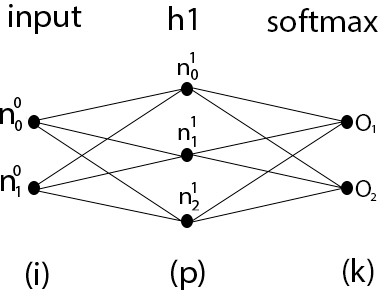
\includegraphics[scale=0.35]{imagenes/nn_1_capa.jpg}  
	\caption{Red Neuronal totalmente conectada con 1 capa oculta}
	\label{fig:nn_1_capa}
\end{figure}

La Figura \ref{fig:nn_1_capa} se compone de 'puntos' interconectados mediante líneas, representando estos neuronas y pesos que las conectan respectivamente. Cada punto corresponde a una neurona, y cada línea a un peso. \\
La Figura \ref{fig:nn_1_capa} presenta 3 capas (input, h1, softmax), que corresponden a la capa de entrada, la capa oculta $h_1$, y la capa de salida, respectivamente. El superíndice indica la capa a la que pertenece una neurona o peso, mientras que el subíndice indica el número del mismo en su respectiva capa. En el caso de los pesos, se requieren 2 subíndices para identificar a cada uno, (cada peso une 2 neuronas). \\
De esta manera, la capa de entrada se compone de 2 neuronas ($n^{0}_0$ y $n^{0}_1$), la capa oculta $h_1$ tiene 3 neuronas ($n^1_{0}$, $n^1_{1}$, y $n^1_{2}$), y el peso $W^{i}_{jk}$ referencia al peso que une las neuronas $n^{i}_j$ y $n^{i+1}_k$.\\
De forma adicional, se recuerda que $Z_i$ representa la entrada $i$ de la capa SoftMax, y, $O_i$, su salida.  

\subsection{Capa SoftMax}

\begin{figure}[H]
	\centering
	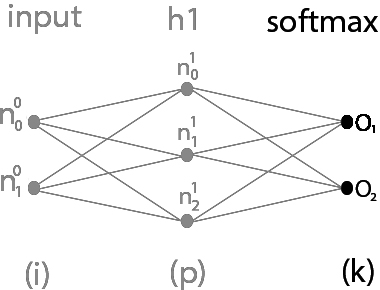
\includegraphics[scale=0.35]{imagenes/nn_1_capa_output.jpg}  
	\caption{Retropropagación en la capa softmax}
	\label{fig:nn_1_capa_output}
\end{figure}

Sea la neurona $n^i_j$, se define como $a^i_j$ el valor de dicha neurona antes de aplicar sobre ella su función de activación asociada, y, $z^i_j$, el obtenido tras aplicarla. 

Tal y como se calculó previamente, el gradiente de la función de pérdida con respecto a cada $Z_i$ viene dado por la fórmula \ref{gradiente_softmax}.


\subsection{Pesos capas h1-SoftMax}

\begin{figure}[H]
	\centering
	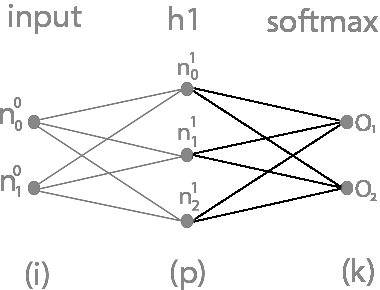
\includegraphics[scale=0.35]{imagenes/nn_1_capa_pesos_h1_output.jpg}  
	\caption{Retropropagación con respecto a pesos entre la capa oculta y la capa SoftMax}
	\label{fig:nn_1_pesos_h1_output}
\end{figure}

Una vez obtenido el gradiente hasta la entrada de la capa softmax, se puede calcular el gradiente con respecto a cada peso $W^1_{pk}$, pues se encuentra conectado a esta desde la capa anterior. Es decir, para cada $h^1_p\in h_1$, se calcula $\frac{dE(x)}{dW^1_{pk}}$. Usando la regla de la cadena, equivale a realizar lo ilustrado en las fórmulas \ref{grad_w1pk_1} y \ref{grad_w1pk_2}.

\begin{gather}
	\frac{\partial Z_k}{\partial W^1_{pk}} = \frac{\partial (z^1_p * W^1 _{pk}+ b^2_k)}{\partial W^1_{pk }} = z^1_p
	\label{grad_w1pk_1}
\end{gather}

\begin{gather}
	\frac{\partial E(x)}{\partial W^1_{pk }} =  gradiente\_Z_k * \frac{\partial Z_k}{\partial W^1_{pk }} = gradiente\_Z_k * z^1_p
	\label{grad_w1pk_2}
\end{gather}

\subsection{Sesgos capa softmax}

Del mismo modo, se calcula el gradiente de la pérdida con respecto a cada sesgo de las neuronas de la capa softmax, tal y como se muestra en las fórmulas \ref{grad_b_h1_1}, \ref{grad_b_h1_2} y \ref{grad_b_h1_3}.

\begin{gather}
	\frac{\partial E}{\partial b^2_k} = \frac{\partial E}{\partial Z_k} * \frac{\partial Z_k}{b^2_k} \label{grad_b_h1_1} \\
	\frac{\partial Z_k }{\partial b^2_k } = \frac{\partial ([\sum_{c=1}^{P} z^1_c * W^1_{pk}] + b^2_k) }{\partial b^2_k } = 1 \label{grad_b_h1_2} \\
	\frac{\partial E}{\partial b^2_k} = gradiente\_Z_k \label{grad_b_h1_3}
\end{gather}

\subsection{Capa oculta h1}

\begin{figure}[H]
	\centering
	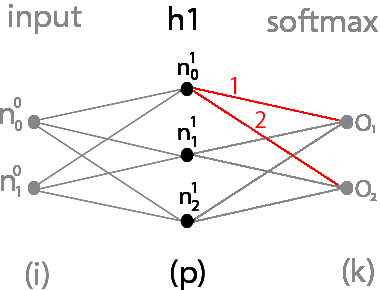
\includegraphics[scale=0.35]{imagenes/nn_caminos_posibles.jpg}  
	\caption{Imagen de los 'caminos' desde la capa softmax hasta la neurona $n^1_0$}
	\label{nn_caminos_posibles}
\end{figure}

En la figura \ref{nn_caminos_posibles}, se muestra como hay más de un 'camino' desde la capa softmax hasta $n^1_p$. Por lo tanto, para obtener el gradiente de la pérdida con respecto a $n^1_p$, es necesario calcular la suma de todos los 'caminos' hacia este, tal y como se presenta en las fórmulas \ref{E_total_a1p} y \ref{deriv_Zk_z1p}. \\

\begin{gather}
	\frac{\partial E_{total}}{\partial a^1_p} = \sum_{k=1}^K \frac{\partial E_k}{\partial a^1_p} = \sum_{k=1}^K  gradiente\_Z_k * \frac{\partial Z_k}{\partial z^1_p} * \frac{\partial z^1_p}{\partial a^1_p}
	\label{E_total_a1p}
\end{gather}

\begin{gather}
	\frac{\partial Z_k}{\partial z^1_p} = \frac{\partial( [\sum_{c=1}^{P} z^1_c * W^1_{ck}] + b^2_k)}{\partial z^1_p} = W^1_{pk}
	\label{deriv_Zk_z1p}
\end{gather}

Para calcular dichos gradientes, se requiere calcular $\frac{\partial z^1_p}{\partial a^1_p}$. Como se mencionó anteriormente, ``a'', se refiere al valor de una neurona antes de aplicar su función de activación asociada, y, ``z'', al valor obtenido tras su aplicación. Por lo tanto, para calcular $\frac{\partial z^1_p}{\partial a^1_p}$, se requiere conocer dicha función de activación.

\begin{figure}[H]
	\centering
	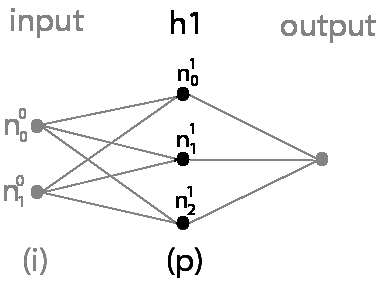
\includegraphics[scale=0.35]{imagenes/nn_1_capa_h1.jpg}  
	\caption{Retropropagación con respecto a neuronas de la capa oculta h1}
	\label{fig:nn_1_capa_h1}
\end{figure}

En este ejemplo, en la capa oculta h1 se emplea la función de activación sigmoide, y su derivada viene dada por las fórmulas \ref{grad_sig_1} y \ref{grad_sig_2}. 

\begin{gather}
	sigmoide(x) = \frac{1}{1+e^{-x}} \label{grad_sig_1} \\
	sigmoide'(x) = \frac{sigmoide(x)}{1-sigmoide(x)} \label{grad_sig_2}
\end{gather}

De este modo, ahora sí se puede calcular $\frac{\partial z^1_p}{\partial a^1_p}$, y se muestra en la fórmula \ref{deriv_z1p_a1p}.

\begin{gather}
	\frac{\partial z^1_ p}{\partial a^1_p} = \frac{\partial sigmoide(a^1_p)}{\partial a^1_p} = sigmoide(a^1_p)*(1-sigmoide(a^1_p))
	\label{deriv_z1p_a1p}
\end{gather}

Así, se retoma la fórmula \ref{E_total_a1p} mediante la aplicación de \ref{deriv_Zk_z1p} y \ref{deriv_z1p_a1p}, y se obtiene \ref{grad_E_a1p}.

\begin{gather}
	\frac{\partial E_{total}}{\partial a^1_p} = \sum_{k=1}^K  gradiente\_Z_k * W^1_{pk} * sigmoide(a^1_p)*(1-sigmoide(a^1_p)) \label{grad_E_a1p} \\
	\frac{\partial E_{total}}{\partial a^1_p} = gradiente\_h1_p \notag
\end{gather}

\subsection{Pesos capas entrada-h1}

Una vez realizada la retropropagación hasta las neuronas de entrada de la capa oculta h1, se puede continuar con el proceso hacia la capa anterior, es decir, la capa de entrada.

\begin{figure}[H]
	\centering
	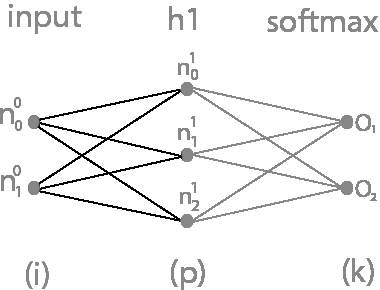
\includegraphics[scale=0.35]{imagenes/nn_1_capa_pesos_input_h1.jpg}  
	\caption{Retropropagación con respecto a los pesos entre la capa de entrada y la capa oculta h1}
	\label{fig:nn_1_pesos_input_h1}
\end{figure}


\begin{gather}
	\frac{\partial a^1_p }{\partial W^0_{ip} } = \frac{\partial [\sum_{c=1}^{I} z^0_c * W^0_{cp}] + b^1_p)}{\partial W^0_{ip} } = z^0_i \label{grad_w0ip_1} \\
	\frac{\partial E}{\partial W^0_{ip}} = \frac{\partial E_{total} }{\partial a^1_p } * \frac{\partial a^1_p}{W^0_{ip}} \label{grad_w0ip_2} \\
	\frac{\partial E(x) }{\partial W^0_{ip} } = gradiente\_h1_p * \frac{\partial a^1_p }{\partial W^0_{ip} } = gradiente\_h1_p * z^0_i 
	\label{grad_w0ip_3}
\end{gather}

De manera similar a como se calcularon los gradientes de la pérdida con respecto a los pesos entre la capa oculta $h_1$ y la capa softmax, se calcula el gradiente de la pérdida con respecto a los pesos entre la capa de entrada y la capa oculta h1. Este proceso se detalla en las fórmulas \ref{grad_w0ip_1}, \ref{grad_w0ip_2}, y \ref{grad_w0ip_3}.

\subsection{Sesgos capa h1}

\begin{gather}
	\frac{\partial E}{\partial b^1_p} = \frac{\partial E_{total} }{\partial a^1_p } * \frac{\partial a^1_p}{b^1_p} \label{grad_b1p_1} \\
	\frac{\partial a^1_p }{\partial b^1_p } = \frac{\partial ([\sum_{c=1}^{I} z^0_c * W^0_{ip}] + b^1_p) }{\partial b^1_p } = 1 \label{grad_b1p_2} \\
	\frac{\partial E}{\partial b^1_p} = gradiente\_h1_p
	\label{grad_b1p_3}
\end{gather}

De manera similar, las figuras \ref{grad_b1p_1}, \ref{grad_b1p_2}, y \ref{grad_b1p_3} ilustran el cálculo del gradiente con respecto a los sesgos de la capa oculta h1.

\subsection{Capa de entrada}

\begin{figure}[H]
	\centering
	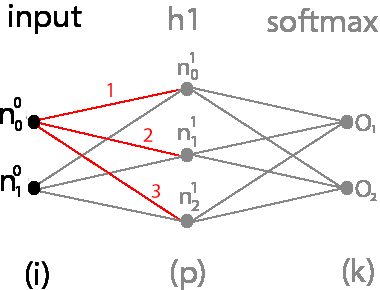
\includegraphics[scale=0.35]{imagenes/nn_caminos_posibles_input.jpg}  
	\caption{Imagen de los 'caminos' desde la capa oculta h1 hasta $n^0_0$}
	\label{nn_caminos_posibles_input}
\end{figure}

Por último, en esta sección se calcula el gradiente con respecto a las neuronas de entrada de la capa de entrada. Aunque, en general, no sería necesario calcular estos gradientes, dado que el objetivo es construir una red neuronal convolucional (CNN), es imprescindible hacerlo. Esto se debe a que la red totalmente conectada estará integrada con capas convolucionales y de agrupación máxima, por lo que es necesario calcular estos gradientes para poder continuar con el proceso de retropropagación en las capas anteriores a esta.

\begin{gather}
	\frac{\partial E_{total}}{\partial a^0_i} = \sum_{p=1}^P \frac{\partial E_{total}}{\partial a^1_p} * \frac{\partial a^1_p}{\partial z^0_i} * \frac{\partial z^0_i}{\partial a^0_i} \notag \\
	\frac{\partial a^1_p }{\partial z^0_i } = \frac{\partial ([\sum_{c=1}^{I} z^0_c * W^0_{ip}] + b^1_p) }{\partial z^0_i } = W^0_{ip} \label{grad_a_2}
\end{gather}

\begin{figure}[H]
	\centering
	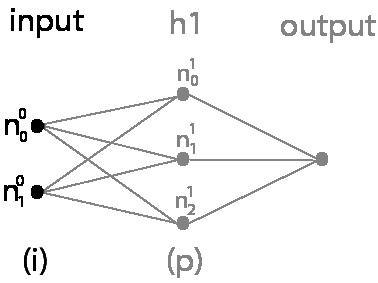
\includegraphics[scale=0.35]{imagenes/nn_1_capa_input.jpg}  
	\caption{Retropropagación en la capa input}
	\label{fig:nn_1_capa_input}
\end{figure}

Como la capa input no presenta ninguna función de activación asociada, se tiene que $z^0_i$ es igual $a^0_i$. \\

\begin{gather}
	\frac{\partial z^0_i }{\partial a^0_i } = 1 \\
	\frac{\partial E_{total}}{\partial a^0_i} = \sum_{p=1}^{P} gradiente\_h1_p
\end{gather}

\section{Retropropagación con 2 capas ocultas}

\begin{figure}[H]
	\centering
	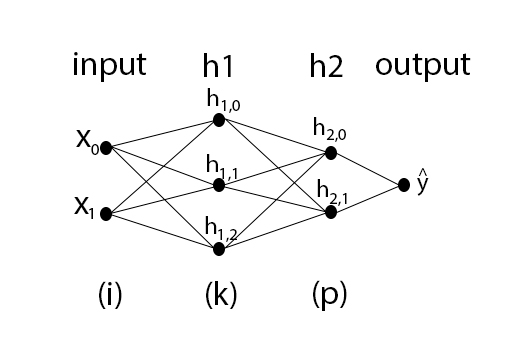
\includegraphics[scale=0.35]{imagenes/nn_2_capas.jpg}  
	\caption{Red Neuronal totalmente conectada con 2 capas ocultas}
	\label{fig:nn_2_capas}
\end{figure}

A diferencia del apartado anterior, en este caso se utiliza una red totalmente conectada con 2 capas ocultas (h1 y h2), tal y como se muestra en la Figura \ref{fig:nn_2_capas}. \\

\subsection{Capa SoftMax}

\begin{figure}[H]
	\centering
	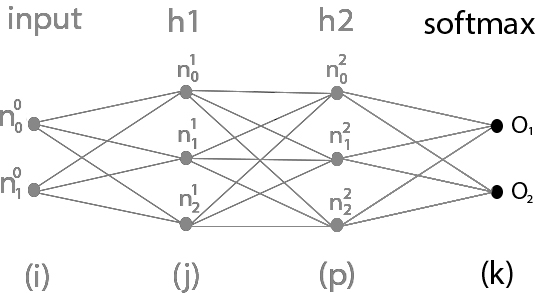
\includegraphics[scale=0.35]{imagenes/nn_2_capa_output.jpg}  
	\caption{Retropropagación en la capa softmax}
\end{figure}

De manera similar a los casos anteriores, el gradiente de la función de pérdida con respecto a cada $Z_i$, se determina mediante la fórmula \ref{gradiente_softmax}. En consecuencia, no se repetirá el cálculo. \\

\subsection{Pesos capas h2-SoftMax}

\begin{figure}[H]
	\centering
	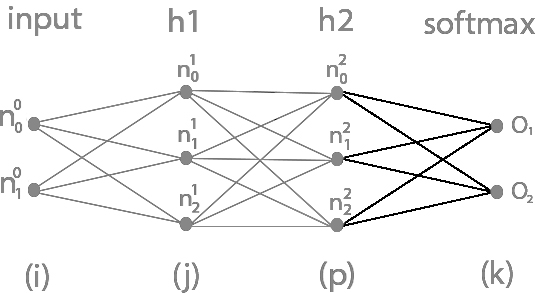
\includegraphics[scale=0.35]{imagenes/nn_2_capa_pesos_h2_output.jpg}  
	\caption{Retropropagación respecto a los pesos entre la capa oculta h2 y la capa SoftMax}
	\label{fig:nn_2_capa_pesos_h2_output}
\end{figure}

Se lleva a cabo el cálculo del gradiente de la función de pérdida con respecto a cada peso $W^2_{pk}$ que conecta las neuronas de la capa oculta h2 con las de la capa softmax (véase la figura \ref{fig:nn_2_capa_pesos_h2_output}). \\

\begin{gather}
	\frac{\partial Z_k}{\partial W^2_{pk}} = \frac{\partial (z^2_p * W^2 _{pk} + b^3_k)}{\partial W^2_{pk }} = z^2_p 
	\label{grad_w2pk_1}
\end{gather}

\begin{gather}
	\frac{\partial E(x)}{\partial W^2_{pk }} =  gradiente\_Z_k * \frac{\partial Z_k}{\partial W^2_{pk }} = gradiente\_Z_k * z^2_p
	\label{grad_w2pk_2}
\end{gather}

Como era de esperar, las fórmulas \ref{grad_w2pk_1} y \ref{grad_w2pk_2} son prácticamente idénticas a las fórmulas \ref{grad_w1pk_1} y \ref{grad_w1pk_2}, respectivamente, con la única diferencia del superíndice empleado (1 $\neq$ 2). Esto resulta lógico, ya que esta parte del cálculo es también común al apartado anterior.

\subsection{Sesgos capa softmax}

\begin{gather}
	\frac{\partial E}{\partial b^3_k} = \frac{\partial E}{\partial Z_k} * \frac{\partial Z_k}{b^3_k} \label{grad_b_h2_1} \\
	\frac{\partial Z_k }{\partial b^3_k } = \frac{\partial ([\sum_{c=1}^{P} z^2_c * W^2_{pk}] + b^3_k) }{\partial b^3_k } = 1 \label{grad_b_h2_2} \\
	\frac{\partial E}{\partial b^3_k} = gradiente\_Z_k \label{grad_b_h2_3}
\end{gather}

De manera similar, el cálculo del gradiente de la pérdida con respecto a los sesgos de la capa softmax también se mantiene inalterado. Por consiguiente, la única diferencia entre las fórmulas $\{$\ref{grad_b_h2_1}, \ref{grad_b_h2_2}, \ref{grad_b_h2_3}$\}$ y $\{$\ref{grad_b_h1_1}, \ref{grad_b_h1_2}, \ref{grad_b_h1_3}$\}$ radica en los superíndices utilizados.

\subsection{Capa oculta h2}

\begin{figure}[H]
	\centering
	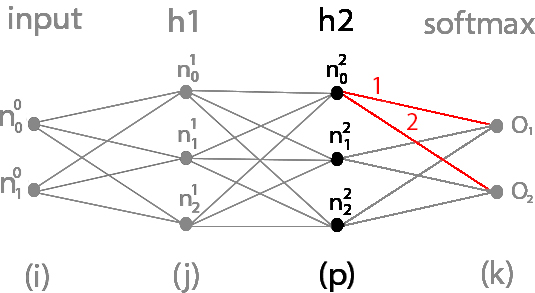
\includegraphics[scale=0.35]{imagenes/nn_h2_caminos_posibles.jpg}  
	\caption{Imagen de los 'caminos' desde la capa softmax hasta $n^2_0$}
	\label{nn_h2_caminos_posibles}
\end{figure}

Tal y como se comentó anteriormente, existen mútiples 'caminos' desde la capa softmax hasta $n^2_p$. Por lo tanto, para obtener el gradiente de la pérdida con respecto a cada $n^2_p$, es necesario calcular la suma de todos ellos, tal y como se detalla en las fórmulas \ref{E_total_a2p} y \ref{deriv_Zk_z2p}. \\

\begin{gather}
	\frac{\partial E_{total}}{\partial a^2_p} = \sum_{k=1}^K \frac{\partial E_k}{\partial a^2_p} = \sum_{k=1}^K  gradiente\_Z_k * \frac{\partial Z_k}{\partial z^2_p} * \frac{\partial z^2_p}{\partial a^2_p}
	\label{E_total_a2p}
\end{gather}

\begin{gather}
	\frac{\partial Z_k}{\partial z^2_p} = \frac{\partial( [\sum_{c=1}^{P} z^2_c * W^2_{ck}] + b^3_k)}{\partial z^2_p} = W^2_{pk}
	\label{deriv_Zk_z2p}
\end{gather}

\begin{figure}[H]
	\centering
	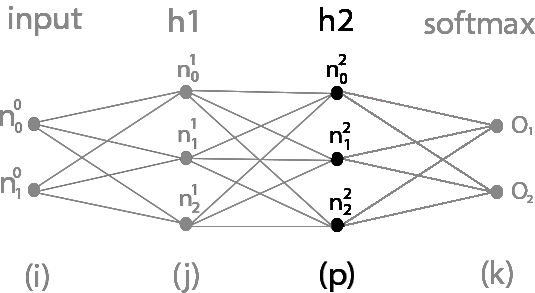
\includegraphics[scale=0.35]{imagenes/nn_2_capa_h2.jpg}  
	\caption{Retropropagación en la capa oculta h2}
	\label{fig:nn_2_capa_h2}
\end{figure}

Dado que coincide con el ejemplo anterior, en la última capa oculta (en este caso, h2), se utiliza nuevamente la función de activación sigmoide. Por lo tanto, se reitera la derivada de esta función en las fórmulas \ref{grad_sig_h2_1} y \ref{grad_sig_h2_2} para facilitar la comprensión del lector.

\begin{gather}
	sigmoide(x) = \frac{1}{1+e^{-x}} \label{grad_sig_h2_1} \\
	sigmoide'(x) = \frac{sigmoide(x)}{1-sigmoide(x)} \label{grad_sig_h2_2}
\end{gather}


Empleando la derivada de sigmoide, se obtiene la fórmula \ref{deriv_z2p_a2p}.

\begin{gather}
	\frac{\partial z^2_ p}{\partial a^2_p} = \frac{\partial sigmoide(a^2_p)}{\partial a^2_p} = sigmoide(a^2_p)*(1-sigmoide(a^2_p))
	\label{deriv_z2p_a2p}
\end{gather}

A continuación, se retoma la fórmula \ref{E_total_a2p} mediante la aplicación de \ref{deriv_Zk_z2p} y \ref{deriv_z2p_a2p} para obtener \ref{grad_E_a2p}.

\begin{gather}
	\frac{\partial E_{total}}{\partial a^2_p} = \sum_{k=1}^K  gradiente\_Z_k * W^2_{pk} * sigmoide(a^2_p)*(1-sigmoide(a^2_p)) \label{grad_E_a2p} \\
	\frac{\partial E_{total}}{\partial a^2_p} = gradiente\_h2_p \notag
\end{gather}

Una vez más, la fórmula obtenida (\ref{grad_E_a2p}) coindice con la calculada previamente (\ref{grad_E_a1p}), salvo por los superíndices empleados. \\

\subsection{Pesos capas h1-h2}

\begin{figure}[H]
	\centering
	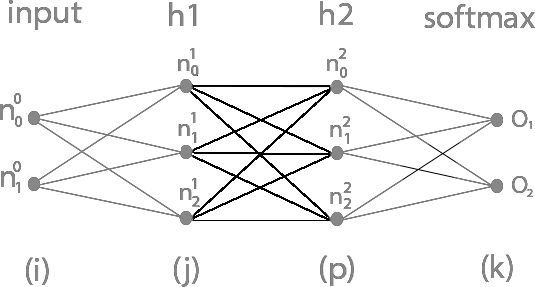
\includegraphics[scale=0.35]{imagenes/nn_2_capa_pesos_h1_h2.jpg}  
	\caption{Retropropagación respecto a los pesos entre las capas ocultas h1 y h2}
	\label{fig:nn_2_pesos_h1_h2}
\end{figure}


\begin{gather}
	\frac{\partial a^2_p }{\partial W^1_{jp} } = \frac{\partial [\sum_{c=1}^{J} z^1_c * W^1_{cp}] + b^2_p)}{\partial W^1_{jp} } = z^1_j \notag \\
	\frac{\partial E}{\partial W^1_{jp}} = \frac{\partial E_{total} }{\partial a^2_p } * \frac{\partial a^2_p}{W^1_{jp}} \notag \\
	\frac{\partial E(x) }{\partial W^1_{jp} } = gradiente\_h2_p * \frac{\partial a^2_p }{\partial W^1_{jp} } = gradiente\_h2_p * z^1_j 
	\label{grad_w1jp}
\end{gather}

Dado que esta parte también es común al caso anterior, la fórmula \ref{grad_w1jp} coincide nuevamente con la fórmula \ref{grad_w0ip_3}.


\subsection{Sesgos capa h2}

\begin{gather}
	\frac{\partial E}{\partial b^2_p} = \frac{\partial E_{total} }{\partial a^2_p } * \frac{\partial a^2_p}{b^2_p} \notag \\
	\frac{\partial a^2_p }{\partial b^2_p } = \frac{\partial ([\sum_{c=1}^{J} z^1_c * W^1_{jp}] + b^2_p) }{\partial b^2_p } = 1 \notag \\
	\frac{\partial E}{\partial b^2_p} = gradiente\_h2_p
	\label{grad_b2p}
\end{gather}

Una vez más, la fórmula \ref{grad_b2p} coincide con \ref{grad_b1p_3}. Es fundamental reconocer las partes comunes entre ambos casos, ya que esto facilita la generalización del modelo y la automatización de los cálculos correspondientes.

\subsection{Capa oculta h1}

\begin{figure}[H]
	\centering
	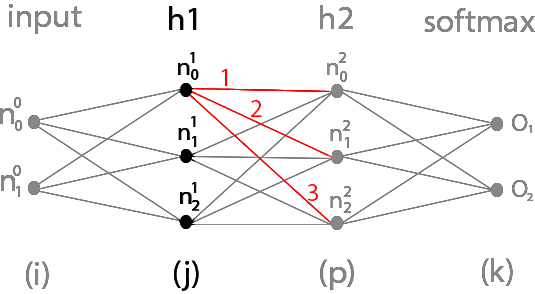
\includegraphics[scale=0.35]{imagenes/nn_h1_caminos_posibles.jpg}  
	\caption{'Caminos' desde la capa softmax hasta $n^1_0$}
	\label{nn_h1_caminos_posibles}
\end{figure}

De manera similar a lo realizado en la capa h2, se calcula la suma de todos los 'caminos' hacia cada neurona $n^1_j$. \\

\begin{gather}
	\frac{\partial E_{total}}{\partial a^1_j} = \sum_{k=1}^K \frac{\partial E_k}{\partial a^1_j} = \sum_{p=1}^P  gradiente\_h2_p * \frac{\partial a^2_p}{\partial z^1_j} * \frac{\partial z^1_j}{\partial a^1_j} \notag \\
	\frac{\partial a^2_p}{\partial z^1_j} = \frac{\partial( [\sum_{c=1}^{J} z^1_c * W^1_{cp}] + b^2_p)}{\partial z^1_j} = W^1_{jp} \notag
\end{gather}

Como era de esperar, se calcula el gradiente con respecto a cada neurona de la capa h1 considerando cada `camino' del gradiente proveniente la capa siguiente (h2).

\begin{figure}[H]
	\centering
	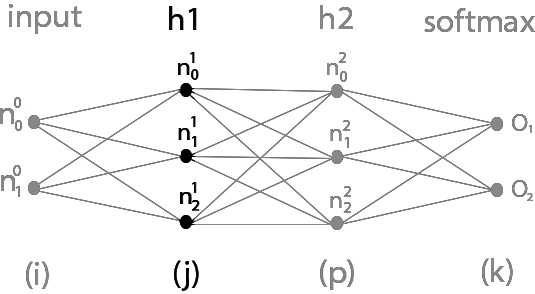
\includegraphics[scale=0.35]{imagenes/nn_2_capa_h1.jpg}  
	\caption{Retropropagación en la capa oculta h1}
\end{figure}

En este caso, en la capa oculta h1 se utiliza la función de activación ReLU, cuya derivada viene dada por la fórmula \ref{deriv_relu}. 

\begin{gather}
	ReLU(x) = max(0, x) \label{relu} \\
	ReLU'(x) = 1\ si\ x>0,\ 0\ en\ caso\ contrario
	\label{deriv_relu}
\end{gather}

La derivada la función de activación ReLU (fórmula \ref{relu}), se emplea para obtener el gradiente $\frac{\partial z^1_ j}{\partial a^1_j}$, y para continuar con la retropropagación a través de la capa, tal y como se detalla en las fórmulas (\ref{grad_E_a1j_1}, \ref{grad_E_a1j_2}, y \ref{grad_E_a1j_3}).


\begin{gather}
	\frac{\partial z^1_ j}{\partial a^1_j} = 1\ si\ x>0,\ 0\ en\ caso\ contrario \label{grad_E_a1j_1} \\
	\frac{\partial E_{total}}{\partial a^1_j} = \sum_{p=1}^P  gradiente\_h2_p * W^1_{jp} * ReLU'(a^1_j) \label{grad_E_a1j_2} \\
	\frac{\partial E_{total}}{\partial a^1_j} = gradiente\_h1_j
	\label{grad_E_a1j_3}
\end{gather}

Una vez más, el proceso para obtener de la fórmula \ref{grad_E_a1j_2} es muy similar al utilizado en casos anteriores, a pesar de que pueda parecer relativamente nueva en comparación con la sección anterior. \\


\subsection{Pesos capa input-h1}

\begin{figure}[H]
	\centering
	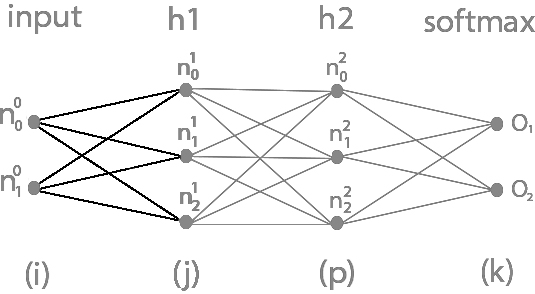
\includegraphics[scale=0.35]{imagenes/nn_2_capa_pesos_input_h1.jpg}  
	\caption{Retropropagación respecto a los pesos entre la capa de entrada y la capa oculta h1}
	\label{fig:nn_2_pesos_input_h1}
\end{figure}


\begin{gather}
	\frac{\partial a^1_j }{\partial W^0_{ij} } = \frac{\partial ([\sum_{c=1}^{I} z^0_c * W^0_{cj}] + b^1_j)}{\partial W^0_{ij} } = z^0_i \label{grad_w0ip_h2_1} \\
	\frac{\partial E}{\partial W^0_{ij}} = \frac{\partial E_{total} }{\partial a^1_j } * \frac{\partial a^1_j}{W^0_{ij}} \label{grad_w0ip_h2_2} \\
	\frac{\partial E(x) }{\partial W^0_{ij} } = gradiente\_h1_j * \frac{\partial a^1_j }{\partial W^0_{ij} } = gradiente\_h1_j * z^0_i \label{grad_w0ip_h2_3}
\end{gather}

Aquí se observa que las fórmulas $\{$\ref{grad_w0ip_h2_1}, \ref{grad_w0ip_h2_2}, \ref{grad_w0ip_h2_3} $\}$ son idénticas a $\{$\ref{grad_w0ip_1}, \ref{grad_w0ip_2}, \ref{grad_w0ip_3} $\}$, excepto por el subíndice empleado (j $\neq$ p). Aunque los valores analíticos puedan diferir debido a las diferencias en las arquitecturas, la notación utilizada se ha diseñado para facilitar la visualización y comprensión de la capacidad de automatización en las capas totalmente conectadas.

\subsection{Sesgos capa h1}

\begin{gather}
	\frac{\partial E}{\partial b^1_j} = \frac{\partial E_{total} }{\partial a^1_j } * \frac{\partial a^1_j}{b^1_j} \label{grad_b1j_h2_1} \\
	\frac{\partial a^1_j }{\partial b^1_j } = \frac{\partial ([\sum_{c=1}^{I} z^0_c * W^0_{ij}] + b^1_j) }{\partial b^1_j } = 1 \label{grad_b1j_h2_2} \\
	\frac{\partial E}{\partial b^1_j} = gradiente\_h1_j
	\label{grad_b1j_h2_3}
\end{gather}

De este modo, las fórmulas $\{$\ref{grad_b1j_h2_1}, \ref{grad_b1j_h2_2}, \ref{grad_b1j_h2_3} $\}$ y $\{$\ref{grad_b1p_1}, \ref{grad_b1p_2}, \ref{grad_b1p_3} $\}$ coinciden en todo los aspectos, excepto en el subíndice (j $\neq$ p).

\subsection{Capa input}

\begin{figure}[H]
	\centering
	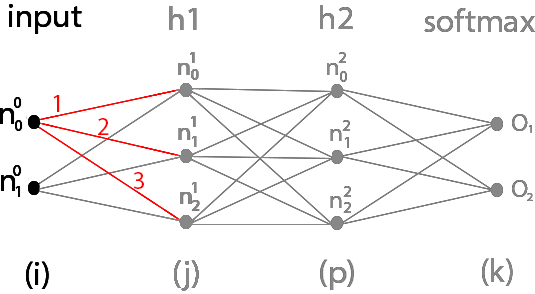
\includegraphics[scale=0.35]{imagenes/nn_2_capas_caminos_posibles_input.jpg}  
	\caption{'Caminos' desde la capa oculta h1 hasta $n^0_0$}
	\label{nn_2_capas_caminos_posibles_input}
\end{figure}

\begin{gather}
	\frac{\partial E_{total}}{\partial a^0_i} = \sum_{j=1}^J \frac{\partial E_{total}}{\partial a^1_j} * \frac{\partial a^1_j}{\partial z^0_i} * \frac{\partial z^0_i}{\partial a^0_i} \label{grad_a_h2_1} \\
	\frac{\partial a^1_j }{\partial z^0_i } = \frac{\partial ([\sum_{c=1}^{I} z^0_c * W^0_{ij}] + b^1_j) }{\partial z^0_i } = W^0_{ij} \label{grad_a_h2_2}
\end{gather}

Aquí también se observa que, a pesar de las diferencias en los subíndices utilizados, las fórmulas $\{$\ref{grad_a_h2_1}, \ref{grad_a_h2_2} $\}$ y $\{$\ref{grad_a_1}, \ref{grad_a_2}$\}$ son idénticas.

\begin{figure}[H]
	\centering
	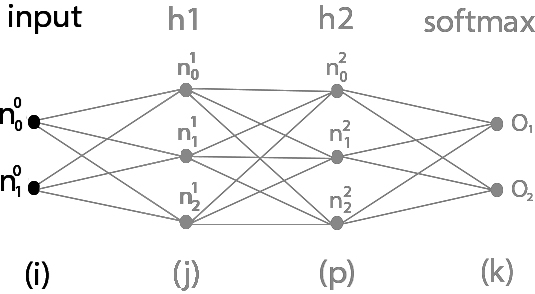
\includegraphics[scale=0.35]{imagenes/nn_2_capa_input.jpg}  
	\caption{Retropropagación en la capa input}
	\label{fig:nn_2_capa_input}
\end{figure}

Dado que la capa de entrada no tiene ninguna función de activación asociada, $z^0_i$ es igual $a^0_i$, al igual que en el caso anterior. \\

\begin{gather}
	\frac{\partial z^0_i }{\partial a^0_i } = 1 \notag \\
	\frac{\partial E_{total}}{\partial a^0_i} = \sum_{p=1}^{P} gradiente\_h1_p \notag
\end{gather}

\section{Conclusiones}
Se definen como capas ocultas ``intermedias'' todas las capas, exceptuando la última de ellas. Tal y como se ha demostrado anteriormente, estas capas comparten la mayoría de los cálculos asociados a la retropropagación. En consecuencia, una red neuronal totalmente conectada puede dividirse en 4 grupos $\{$capa de entrada, capas ocultas intermedias, última capa oculta, capa de salida o capa softmax$\}$. \\
A continuación se realiza el cálculo necesario para la retropropagación de una capa de neuronas \textit{l} específica. Suponemos que la capa \textit{l+1} tiene \textit{Q} neuronas, la capa \textit{l-1} tiene \textit{K} neuronas, y que todas las capas ocultas intermedias usan ReLU como función de activación. \\

\subsection{Gradiente respecto a la entrada de la capa}

\begin{figure}[H]
	\centering
	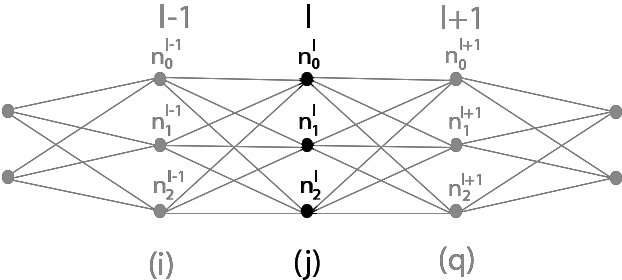
\includegraphics[scale=0.35]{imagenes/conclusion_capa_l.jpg}  
	\caption{Retropropagación en la capa l}
	\label{fig:conclusion_capa_l_apendice}
\end{figure}

\begin{gather}
	\frac{\partial E_{total}}{\partial a^l_j} = \sum_{q=1}^Q \frac{\partial E_{total}}{\partial a^{l+1}_q} * \frac{\partial a^{l+1}_q}{\partial z^l_j} * \frac{\partial z^l_j}{\partial a^l_j} \label{grad_input_l_1} \\
	\frac{\partial a^{l+1}_j }{\partial z^l_j } = \frac{\partial ([\sum_{c=1}^{K} z^l_c * W^l_{ij}] + b^{l+1}_j) }{\partial z^l_j } = W^l_{ij} \label{grad_input_l_2} \\
	\frac{\partial z^l_j}{\partial a^l_j} = ReLU'(a^l_j) \label{grad_input_l_3} \\
	\frac{\partial E_{total}}{\partial a^l_j} = \sum_{q=1}^Q  gradiente\_h_{{l+1}_q} * W^l_{ij} * ReLU'(a^l_j) \label{grad_input_l_4_apendice} \\
	\frac{\partial E_{total}}{\partial a^l_j} = gradiente\_h_{l_j} \label{grad_input_l_5}
\end{gather}

Las fórmulas \ref{grad_input_l_1}, \ref{grad_input_l_2}, \ref{grad_input_l_3},  \ref{grad_input_l_4_apendice}, y \ref{grad_input_l_5}, ilustran el cálculo genérico necesario para obtener el gradiente de la pérdida con respecto a la entrada de una capa oculta intermedia \textit{l}.

\subsection{Gradiente respecto a los pesos}

\begin{figure}[H]
	\centering
	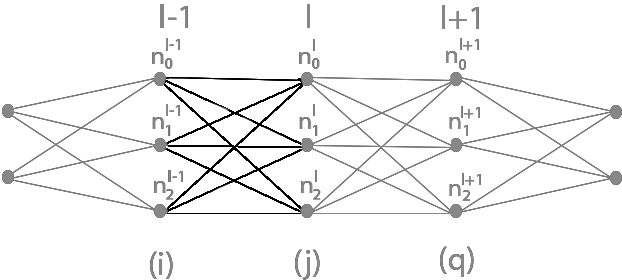
\includegraphics[scale=0.35]{imagenes/conclusion_pesos.jpg}  
	\caption{Retropropagación respecto a los pesos entre la capa l-1 y l}
	\label{fig:conclusion_pesos_apendice}
\end{figure}

\begin{gather}
	\frac{\partial E}{\partial W^{l-1}_{ij}} = \frac{\partial E_{total} }{\partial a^l_j } * \frac{\partial a^l_j}{W^{l-1}_{ij}} \label{grad_w_l_1} \\
	\frac{\partial a^l_j }{\partial W^{l-1}_{ij} } = \frac{\partial ([\sum_{c=1}^{K} z^{l-1}_c * W^{l-1}_{cj}] + b^l_j)}{\partial W^{l-1}_{ij} } = z^{l-1}_i \label{grad_w_l_2} \\
	\frac{\partial E(x) }{\partial W^{l-1}_{ij} } = gradiente\_h_{l_j} * \frac{\partial a^l_j }{\partial W^{l-1}_{ij} } = gradiente\_h_{l_j} * z^{l-1}_i \label{grad_w_l_3_apendice}
\end{gather}

Las fórmulas \ref{grad_w_l_1}, \ref{grad_w_l_2}, y \ref{grad_w_l_3_apendice} detallan el cálculo necesario para determinar el gradiente de la pérdida con respecto a los pesos entre las capas ocultas \textit{l} y \textit{l-1}.

\subsection{Gradiente respecto a sesgos}

\begin{gather}
	\frac{\partial E}{\partial b^l_j} = \frac{\partial E_{total} }{\partial a^l_j } * \frac{\partial a^l_j}{b^l_j} \label{grad_b_l_1} \\
	\frac{\partial a^l_j }{\partial b^l_j } = \frac{\partial ([\sum_{c=1}^{K} z^{l-1}_c * W^{l-1}_{ij}] + b^l_j) }{\partial b^l_j } = 1 \label{grad_b_l_2} \\
	\frac{\partial E}{\partial b^l_j} = gradiente\_h_{l_j} \label{grad_b_l_3_apendice}
\end{gather}

Las fórmulas \ref{grad_b_l_1}, \ref{grad_b_l_2}, y \ref{grad_b_l_3_apendice} presentan el cálculo necesario para obtener el gradiente de la pérdida con respecto a los sesgos de la capa oculta \textit{l}.

\chapter{Retropropagación en capas convolucionales} \label{backprop_conv_apendice}

\begin{figure}[H]
	\centering
	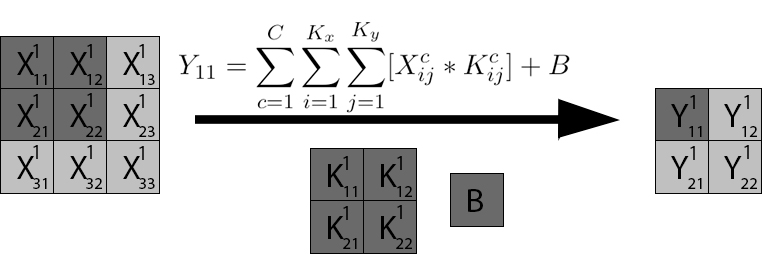
\includegraphics[width=0.8\linewidth]{imagenes/conv_ejemplo_backprop_1.jpg} 
	\caption{Ejemplo de propagación hacia delante en una capa convolucional}
	\label{fig:ejemplo_forward_prop_convolucional_apendice}
\end{figure}

La figura \ref{fig:ejemplo_forward_prop_convolucional_apendice} ilustra el ejemplo de propagación hacia delante que se utilizará en esta sección. En dicha figura, \textit{C} representa el número de canales de profundidad del volumen de entrada \textit{X}, mientras que ${K_x}$ y ${K_y}$ se refieren al número de filas y columnas del kernel \textit{K} utilizado, respectivamente. \\
Siguiendo la notación empleada en secciones anteriores, se denotará por $A^c_{ij}$ al valor de $X^c_{ij}$ antes de aplicar la función de activación correspondiente, y por $Z^c_{ij}$, al valor resultante después de aplicar dicha función.

\section{Sumatoria de gradientes}

\begin{gather}
	\frac{\partial E}{\partial K^c_{11}} = \sum_{i=1}^{I}\sum_{j=1}^{J}  [\frac{\partial E}{\partial Y^c_{ij}} \frac{\partial Y^c_{ij}}{\partial K^c_{11}}] \\
	\frac{\partial E}{\partial X^c_{11}} = \sum_{i=1}^{I}\sum_{j=1}^{J}  [\frac{\partial E}{\partial Y^c_{ij}} \frac{\partial Y^c_{ij}}{\partial Z^c_{11}} \frac{\partial Z^c_{ij}}{\partial A^c_{11}}] 
\end{gather}

Para calcular el gradiente de la función de error con respecto a cada peso ${K_{xy}}$ o entrada ${X_{xy}}$, se debe realizar una sumatoria del gradiente correspondiente sobre cada valor de salida producido por la convolución. En el caso de los pesos asociados a un canal de profundidad $c \in C$, cada peso ${K_{xy}}$ se empleó en el cálculo de cada valor $Y^c_{ij}$. Por otro lado, los valores de la entrada ${X_{xy}}$ contribuyen al cálculo de varios valores de salida $\{Y_1, Y_2\} \in Y$. Este proceso fue detallado anteriormente en la sección \ref{intro_CNN}.

\subsection{Gradiente de $Y^c_{11}$}

\begin{gather}
	Y^c_{11} = Z^c_{11} K^c_{11} + Z^c_{12} K^c_{12} + Z^c_{21} K^c_{21} + Z^c_{22} K^c_{22} \label{grad_y11_k_11_apendice} \\
	\frac{\partial Y^c_{11}}{\partial K^c_{xy}} = \frac{\partial (Z^c_{11} K^c_{11} + Z^c_{12} K^c_{12} + Z^c_{21} K^c_{21} + Z^c_{22} K^c_{22})}{\partial K^c_{xy}} \label{grad_y11_k_12_apendice} \\
	\frac{\partial Y^c_{11}}{\partial K^c_{11}} = Z^c_{11}, \hspace{10mm} \frac{\partial Y^c_{11}}{\partial K^c_{12}} = Z^c_{12} \label{grad_y11_k_21_apendice}\\
	\frac{\partial Y^c_{11}}{\partial K^c_{21}} = Z^c_{21}, \hspace{10mm} \frac{\partial Y^c_{11}}{\partial K^c_{22}} = Z^c_{22} \label{grad_y11_k_22_apendice}
\end{gather}

\begin{gather}
	\frac{\partial Y^c_{11}}{\partial Z^c_{11}} = K^c_{11}, \hspace{10mm} \frac{\partial Y^c_{11}}{\partial Z^c_{12}} = K^c_{12}, \hspace{10mm} \frac{\partial Y^c_{11}}{\partial Z^c_{13}} = 0 \label{grad_y11_z_1} \\
	\frac{\partial Y^c_{11}}{\partial Z^c_{21}} = K^c_{21}, \hspace{10mm} \frac{\partial Y^c_{11}}{\partial Z^c_{22}} = K^c_{22}, \hspace{10mm} \frac{\partial Y^c_{11}}{\partial Z^c_{23}} = 0 \label{grad_y11_z_2} \\
	\frac{\partial Y^c_{11}}{\partial Z^c_{31}} = 0, \hspace{15mm} \frac{\partial Y^c_{11}}{\partial Z^c_{32}} = 0, \hspace{15mm} \frac{\partial Y^c_{11}}{\partial Z^c_{33}} = 0 \label{grad_y11_z_3}
\end{gather}

La fórmula \ref{grad_y11_k_11_apendice}, presenta una descomposición de $Y^c_{11}$ en términos de $Z$ y $K$. Esto, es esencial para el cálculo del gradiente, tanto con respecto a Z, (como se detalla en las fórmulas \ref{grad_y11_z_1}, \ref{grad_y11_z_2}, \ref{grad_y11_z_3}), como con respecto a K, (como se muestra en las fórmulas \ref{grad_y11_k_12_apendice}, \ref{grad_y11_k_21_apendice}, \ref{grad_y11_k_22_apendice}). Esta descomposición, permite calcular el gradiente de $Y^c_{11}$ con respecto a cada parámetro de la capa convolucional. \\
Cabe destacar que, para calcular el gradiente con respecto a cada valor del volumen de entrada (X), también debe calcularse la derivada de la función de activación asociada a dicha capa. Es decir, $\frac{\partial Z}{\partial A}$. Sin embargo, dado que este proceso ha sido abordado en secciones anteriores, se omitirá en esta ocasión, al igual que el cálculo del gradiente con respecto al sesgo de cada capa. El propósito de esta omisión es evitar cálculos redundantes y concentrar la atención en los aspectos más relevantes e innovadores. No obstante, es importante señalar que todos los cálculos discutidos en esta documentación, y más, están implementados en el código correspondiente, lo que garantiza que este conocimiento se ha aplicado y verificado en la práctica. \\
Además, dado que todo ha sido realizado manualmente por la misma persona, la mayoría de las variables e índices utilizados en la documentación coinciden perfectamente o son muy similares a los empleados en el código. Esto asegura que cualquier lector con conocimientos básicos de programación pueda comprender gran parte de las implementaciones desarrolladas en este proyecto.

\subsection{Gradiente de $Y^c_{12}$}

\begin{figure}[H]
	\centering
	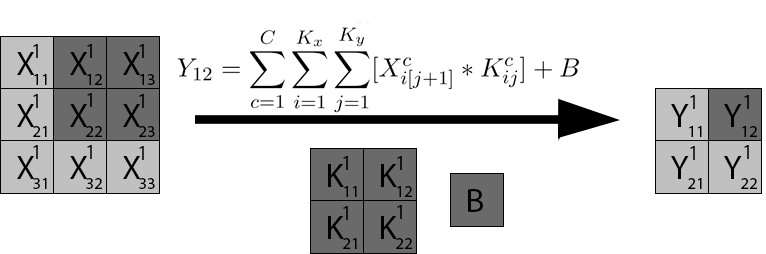
\includegraphics[width=1\linewidth]{imagenes/conv_ejemplo_backprop_2.jpg} 
	\caption{Cálculo de $Y^c_{12}$ mediante propagación hacia delante en una capa convolucional}
	\label{fig:ejemplo_2_forward_prop_convolucional}
\end{figure}

Del mismo modo, se calcula el gradiente de $Y^c_{12}$ con respecto a cada peso, como se muestra en las fórmulas \ref{grad_y12_k_1} y \ref{grad_y12_k_2}.

\begin{gather}
	Y^c_{12} = Z^c_{12}   K^c_{11} + Z^c_{13}   K^c_{12} + Z^c_{22}   K^c_{21} + Z^c_{23}   K^c_{22} \\
	\frac{\partial Y^c_{12}}{\partial K^c_{xy}} = \frac{\partial (Z^c_{11}   K^c_{11} + Z^c_{12}   K^c_{12} + Z^c_{21}   K^c_{21} + Z^c_{22}   K^c_{22})}{\partial K^c_{xy}} \\
	\frac{\partial Y^c_{12}}{\partial K^c_{11}} = Z^c_{12}, \hspace{10mm} \frac{\partial Y^c_{12}}{\partial K^c_{12}} = Z^c_{13} \label{grad_y12_k_1} \\
	\frac{\partial Y^c_{12}}{\partial K^c_{21}} = Z^c_{22}, \hspace{10mm} \frac{\partial Y^c_{12}}{\partial K^c_{22}} = Z^c_{23} \label{grad_y12_k_2}
\end{gather}

Asimismo, se calcula el gradiente de $Y^c_{12}$ con respecto a cada valor de entrada, como se detalla en las fórmulas \ref{grad_y12_z_1}, \ref{grad_y12_z_2} y \ref{grad_y12_z_3}.

\begin{gather}
	\frac{\partial Y^c_{12}}{\partial Z^c_{11}} = 0, \hspace{10mm} \frac{\partial Y^c_{12}}{\partial Z^c_{12}} = K^c_{11}, \hspace{10mm} \frac{\partial Y^c_{12}}{\partial Z^c_{13}} = K^c_{12} \label{grad_y12_z_1} \\
	\frac{\partial Y^c_{12}}{\partial Z^c_{21}} = 0, \hspace{10mm} \frac{\partial Y^c_{12}}{\partial Z^c_{22}} = K^c_{21}, \hspace{10mm} \frac{\partial Y^c_{12}}{\partial Z^c_{23}} = K^c_{22} \label{grad_y12_z_2} \\
	\frac{\partial Y^c_{12}}{\partial Z^c_{31}} = 0, \hspace{10mm} \frac{\partial Y^c_{12}}{\partial Z^c_{32}} = 0, \hspace{15mm} \frac{\partial Y^c_{12}}{\partial Z^c_{33}} = 0 \hspace{5mm} \label{grad_y12_z_3}
\end{gather}

\subsection{Gradiente de $Y^c_{21}$}

\begin{figure}[H]
	\centering
	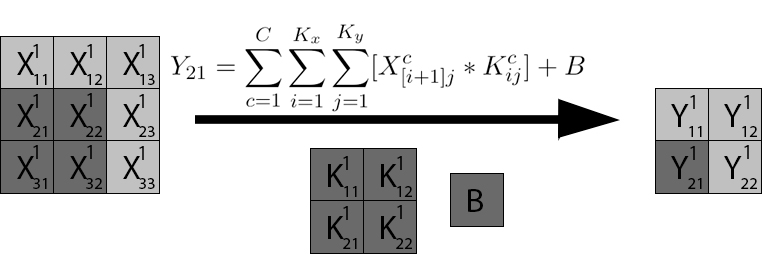
\includegraphics[width=1\linewidth]{imagenes/conv_ejemplo_backprop_3.jpg} 
	\caption{Cálculo de $Y^c_{21}$ mediante propagación hacia delante en una capa convolucional}
	\label{fig:ejemplo_3_forward_prop_convolucional}
\end{figure}

Se calcula el gradiente de $Y^c_{21}$ con respecto a cada peso, tal y como se muestra en las ecuaciones \ref{grad_y21_k_1} y \ref{grad_y21_k_2}.

\begin{gather}
	Y^c_{21} = Z^c_{21}   K^c_{11} + Z^c_{22}   K^c_{12} + Z^c_{31}   K^c_{21} + Z^c_{32}   K^c_{22} \\
	\frac{\partial Y^c_{21}}{\partial K^c_{xy}} = \frac{\partial (Z^c_{21}   K^c_{11} + Z^c_{22}   K^c_{12} + Z^c_{31}   K^c_{21} + Z^c_{32}   K^c_{22})}{\partial K^c_{xy}} \\
	\frac{\partial Y^c_{21}}{\partial K^c_{11}} = Z^c_{21}, \hspace{10mm} \frac{\partial Y^c_{21}}{\partial K^c_{12}} = Z^c_{22} \label{grad_y21_k_1} \\
	\frac{\partial Y^c_{21}}{\partial K^c_{21}} = Z^c_{31}, \hspace{10mm} \frac{\partial Y^c_{21}}{\partial K^c_{22}} = Z^c_{32} \label{grad_y21_k_2}
\end{gather}

Asimismo, se calcula el gradiente de $Y^c_{21}$ con respecto a cada valor de entrada, según se detalla en las ecuaciones \ref{grad_y21_z_1}, \ref{grad_y21_z_2} y \ref{grad_y21_z_3}.

\begin{gather}
	\frac{\partial Y^c_{21}}{\partial Z^c_{11}} = 0, \hspace{16mm} \frac{\partial Y^c_{21}}{\partial Z^c_{12}} = 0, \hspace{13mm} \frac{\partial Y^c_{21}}{\partial Z^c_{13}} = 0 \label{grad_y21_z_1} \\
	\frac{\partial Y^c_{21}}{\partial Z^c_{21}} = K^c_{11}, \hspace{10mm} \frac{\partial Y^c_{21}}{\partial Z^c_{22}} = K^c_{12}, \hspace{10mm} \frac{\partial Y^c_{21}}{\partial Z^c_{23}} = 0 \label{grad_y21_z_2} \\
	\frac{\partial Y^c_{21}}{\partial Z^c_{31}} = K^c_{21}, \hspace{10mm} \frac{\partial Y^c_{21}}{\partial Z^c_{32}} = K^c_{22}, \hspace{10mm} \frac{\partial Y^c_{21}}{\partial Z^c_{33}} = 0 \label{grad_y21_z_3}
\end{gather}


\subsection{Gradiente de $Y^c_{22}$}

\begin{figure}[H]
	\centering
	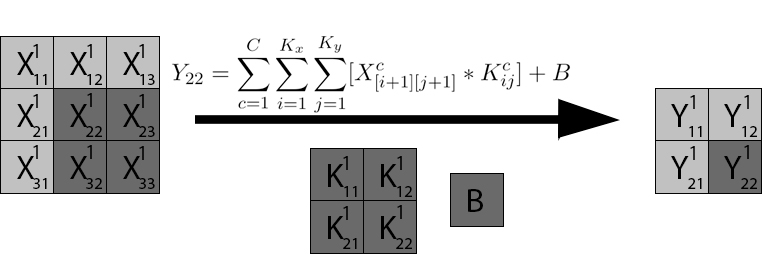
\includegraphics[width=1\linewidth]{imagenes/conv_ejemplo_backprop_4.jpg} 
	\caption{Cálculo de $Y^c_{22}$ mediante propagación hacia delante en una capa convolucional}
	\label{fig:ejemplo_4_forward_prop_convolucional}
\end{figure}

El gradiente de $Y^c_{22}$ se calcula con respecto a cada peso, como se muestra en las fórmulas \ref{grad_y22_k_1} y \ref{grad_y22_k_2}.

\begin{gather}
	Y^c_{22} = Z^c_{22}   K^c_{11} + Z^c_{23}   K^c_{12} + Z^c_{32}   K^c_{21} + Z^c_{33}   K^c_{22} \\
	\frac{\partial Y^c_{22}}{\partial K^c_{xy}} = \frac{\partial (Z^c_{11}   K^c_{11} + Z^c_{12}   K^c_{12} + Z^c_{21}   K^c_{21} + Z^c_{22}   K^c_{22})}{\partial K^c_{xy}} \\
	\frac{\partial Y^c_{22}}{\partial K^c_{11}} = Z^c_{22}, \hspace{10mm} \frac{\partial Y^c_{22}}{\partial K^c_{12}} = Z^c_{23} \label{grad_y22_k_1} \\
	\frac{\partial Y^c_{22}}{\partial K^c_{21}} = Z^c_{32}, \hspace{10mm} \frac{\partial Y^c_{22}}{\partial K^c_{22}} = Z^c_{33} \label{grad_y22_k_2}
\end{gather}

Se calcula el gradiente de $Y^c_{22}$ respecto a cada valor del volumen de entrada, como se muestra en las fórmulas \ref{grad_y22_z_1}, \ref{grad_y22_z_2}, y \ref{grad_y22_z_3}.

\begin{gather}
	\frac{\partial Y^c_{22}}{\partial Z^c_{11}} = 0, \hspace{10mm} \frac{\partial Y^c_{22}}{\partial Z^c_{12}} = 0, \hspace{15mm} \frac{\partial Y^c_{22}}{\partial Z^c_{13}} = 0 \hspace{4mm} \label{grad_y22_z_1} \\
	\frac{\partial Y^c_{22}}{\partial Z^c_{21}} = 0, \hspace{10mm} \frac{\partial Y^c_{22}}{\partial Z^c_{22}} = K^c_{11}, \hspace{10mm} \frac{\partial Y^c_{22}}{\partial Z^c_{23}} = K^c_{12} \label{grad_y22_z_2} \\
	\frac{\partial Y^c_{22}}{\partial Z^c_{31}} = 0, \hspace{10mm} \frac{\partial Y^c_{22}}{\partial Z^c_{32}} = K^c_{21}, \hspace{10mm} \frac{\partial Y^c_{22}}{\partial Z^c_{33}} = K^c_{22} \label{grad_y22_z_3}
\end{gather}

\subsection{Gradiente respecto a pesos como convolución}

Finalmente, se procede al cálculo de la suma total de gradientes con respecto a cada peso de la capa, conforme a las fórmulas \ref{grad_Y_K_1_apendice}, \ref{grad_Y_K_2_apendice}, \ref{grad_Y_K_3_apendice}, y \ref{grad_Y_K_4_apendice}. Se observa un patrón claro en los gradientes resultantes, que refleja la contribución de cada peso en el cálculo del error total.

\begin{gather}
	\frac{\partial E}{\partial K^c_{11}} = \frac{\partial E}{\partial Y^c_{11}}   Z^c_{11} + \frac{\partial E}{\partial Y^c_{12}}   Z^c_{12} + \frac{\partial E}{\partial Y^c_{21}}   Z^c_{21} + \frac{\partial E}{\partial Y^c_{22}}   Z^c_{22} \label{grad_Y_K_1_apendice} \\
	\frac{\partial E}{\partial K^c_{12}} = \frac{\partial E}{\partial Y^c_{11}}   Z^c_{12} + \frac{\partial E}{\partial Y^c_{12}}   Z^c_{13} + \frac{\partial E}{\partial Y^c_{21}}   Z^c_{22} + \frac{\partial E}{\partial Y^c_{22}}   Z^c_{23} \label{grad_Y_K_2_apendice} \\	
	\frac{\partial E}{\partial K^c_{21}} = \frac{\partial E}{\partial Y^c_{11}}   Z^c_{21} + \frac{\partial E}{\partial Y^c_{12}}   Z^c_{22} + \frac{\partial E}{\partial Y^c_{31}}   Z^c_{21} + \frac{\partial E}{\partial Y^c_{22}}   Z^c_{32} \label{grad_Y_K_3_apendice} \\
	\frac{\partial E}{\partial K^c_{22}} = \frac{\partial E}{\partial Y^c_{11}}   Z^c_{22} + \frac{\partial E}{\partial Y^c_{12}}   Z^c_{23} + \frac{\partial E}{\partial Y^c_{31}}   Z^c_{32} + \frac{\partial E}{\partial Y^c_{22}}   Z^c_{33} \label{grad_Y_K_4_apendice}
\end{gather}

Como se observa en los cálculos realizados, estos coinciden con una operación de convolución entre la entrada \textit{X} y el gradiente respecto a la capa de salida \textit{Y}. Este procedimiento se detalla en la Figura \ref{fig:conv_backprop_como_convolucion_X_Y_apendice} \cite{conv_backprop}.

\begin{figure}[H]
	\centering
	\begin{subfigure}{.5\textwidth}
		\hspace{-25mm}
		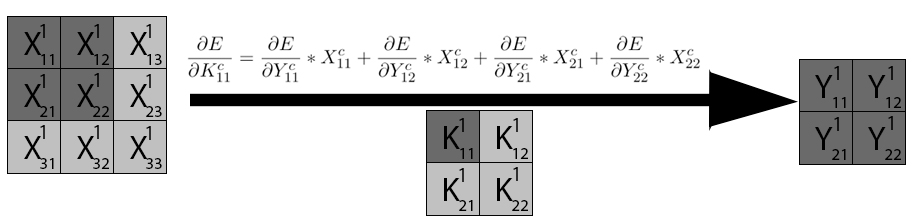
\includegraphics[width=1.4\linewidth]{imagenes/conv_backprop_1.jpg}  
		\caption{Cálculo de $\frac{\partial E}{\partial K^1_{11}}$}
	\end{subfigure}%
	\begin{subfigure}{.5\textwidth}
		\hspace{5mm}
		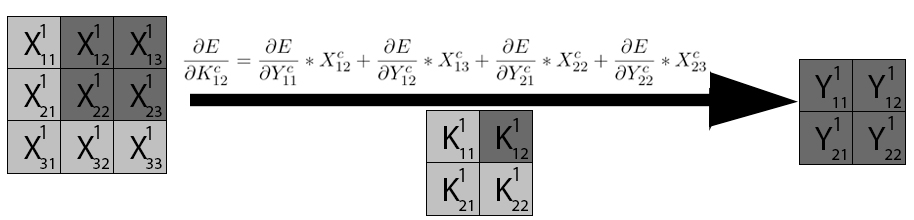
\includegraphics[width=1.4\linewidth]{imagenes/conv_backprop_2.jpg}  
		\caption{Cálculo de $\frac{\partial E}{\partial K^1_{12}}$}
	\end{subfigure}
	\vspace{5mm}
	\begin{subfigure}{.5\textwidth}
		\hspace{-25mm}
		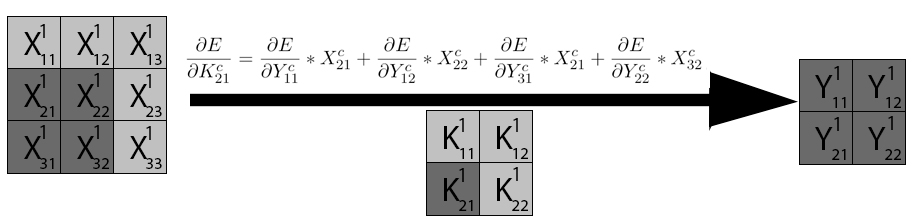
\includegraphics[width=1.4\linewidth]{imagenes/conv_backprop_3.jpg}  
		\caption{Cálculo de $\frac{\partial E}{\partial K^1_{21}}$}
	\end{subfigure}%
	\begin{subfigure}{.5\textwidth}
		\hspace{5mm}
		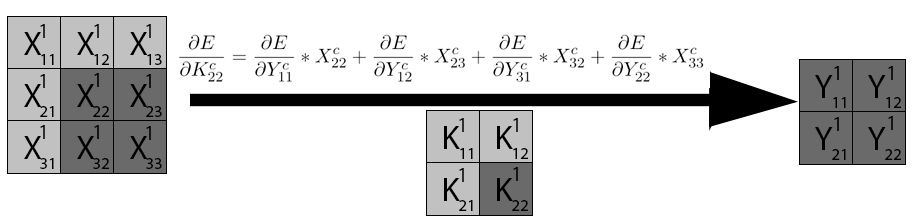
\includegraphics[width=1.4\linewidth]{imagenes/conv_backprop_4.jpg}  
		\caption{Cálculo de $\frac{\partial E}{\partial K^1_{22}}$}
	\end{subfigure}
	\caption{Cálculo del gradiente de la pérdida con respecto a cada filtro como convolución entre X e Y}
	\label{fig:conv_backprop_como_convolucion_X_Y_apendice}
\end{figure}

En la figura \ref{fig:conv_backprop_como_convolucion_X_Y_apendice}, cada subfigura $\{(a), (b), (c), (d)\}$ representa el cálculo del gradiente con respecto a un peso específico. Aunque la representación puede parecer algo diferente a simple vista, los cálculos son esencialmente los mismos que los obtenidos anteriormente, con la única diferencia en la forma en que se visualizan.

\subsection{Gradiente respecto a entrada como convolución}

Por razones de simplicidad, y en consonancia con las recomendaciones de expertos, y la experiencia personal, se empleará ReLU como función de activación en las capas convolucionales. Dado que, la derivada de esta función ya ha sido previamente calculada, (véase la fórmula \ref{deriv_relu}), se considerará esta información para los cálculos subsiguientes.


\begin{gather}
	\frac{\partial E}{\partial A^c_{11}} = \frac{\partial E}{\partial Y^c_{11}}   K^c_{11}    ReLU'(A^c_{11}) \\
	\frac{\partial E}{\partial A^c_{12}} = (\frac{\partial E}{\partial Y^c_{11}}   K^c_{12} + \frac{\partial E}{\partial Y^c_{12}}   K^c_{11})   ReLU'(A^c_{12}) \\
	\frac{\partial E}{\partial A^c_{13}} = \frac{\partial E}{\partial Y^c_{12}}   K^c_{12}   ReLU'(A^c_{13}) \\
\end{gather}

\begin{gather}
	\frac{\partial E}{\partial A^c_{21}} = (\frac{\partial E}{\partial Y^c_{11}}   K^c_{21} + \frac{\partial E}{\partial Y^c_{21}}   K^c_{11})   ReLU'(A^c_{21}) \\
	\frac{\partial E}{\partial A^c_{22}} = (\frac{\partial E}{\partial Y^c_{11}}   K^c_{22} + \frac{\partial E}{\partial Y^c_{12}}   K^c_{21} + \frac{\partial E}{\partial Y^c_{21}}   K^c_{12} + \frac{\partial E}{\partial Y^c_{22}}   K^c_{11})   ReLU'(A^c_{22}) \\
	\frac{\partial E}{\partial A^c_{23}} = (\frac{\partial E}{\partial Y^c_{12}}   K^c_{22} + \frac{\partial E}{\partial Y^c_{22}}   K^c_{12})   ReLU'(A^c_{22})\\
\end{gather}

\begin{gather}
	\frac{\partial E}{\partial A^c_{31}} = \frac{\partial E}{\partial Y^c_{21}}   K^c_{21}   ReLU'(A^c_{31})\\
	\frac{\partial E}{\partial A^c_{32}} = (\frac{\partial E}{\partial Y^c_{21}}   K^c_{22} + \frac{\partial E}{\partial Y^c_{22}}   K^c_{21})   ReLU'(A^c_{32})\\
	\frac{\partial E}{\partial A^c_{33}} = \frac{\partial E}{\partial Y^c_{22}}   K^c_{22}   ReLU'(A^c_{33})
\end{gather}

Tal y como se observa en los cálculos obtenidos, estos corresponden a una convolución de tipo ``full'' (completa) entre el gradiente con respecto a la capa de salida (Y) y los pesos (K), invertidos tanto horizontal como verticalmente. El proceso de cálculo del gradiente con respecto a cada valor $x \in X$ se presenta en detalle en la figura \ref{fig:conv_backprop_como_convolucion_Y_W_apendice}, mientras que la manera de invertir los pesos se ilustra en la figura \ref{fig:flip_W_apendice} \cite{conv_backprop}.

\begin{figure}[H]
	\centering
	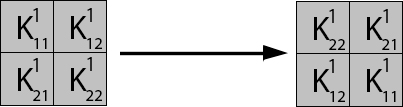
\includegraphics[width=0.8\linewidth]{imagenes/flip_pesos.jpg}  
	\caption{Inversión de los pesos en K tanto horizontal como verticalmente}
	\label{fig:flip_W_apendice}
\end{figure}

\begin{figure}[H]
	\centering
	\begin{subfigure}{.5\textwidth}
		\hspace{-25mm}
		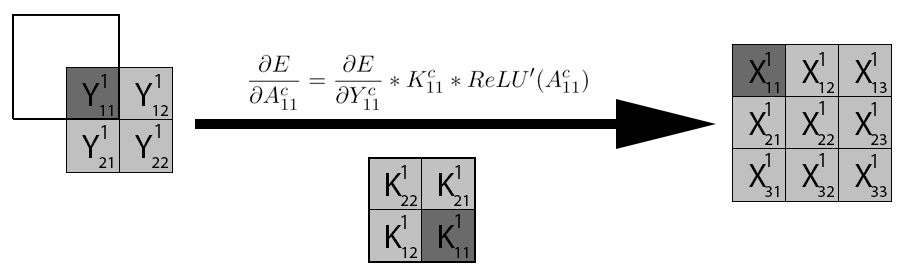
\includegraphics[width=1.4\linewidth]{imagenes/conv_back_entrada_1.jpg}  
		\caption{Gradiente con respecto a $X^1_{11}$}
	\end{subfigure}%
	\begin{subfigure}{.5\textwidth}
		\hspace{5mm}
		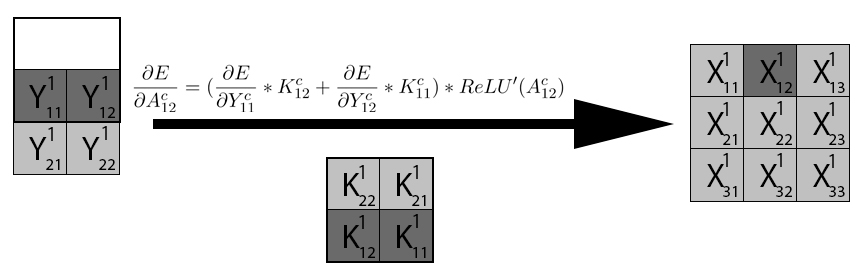
\includegraphics[width=1.4\linewidth]{imagenes/conv_back_entrada_2.jpg}  
		\caption{Gradiente con respecto a $X^1_{12}$}
	\end{subfigure}
	\vspace{5mm}
	\begin{subfigure}{.5\textwidth}
		\hspace{-25mm}
		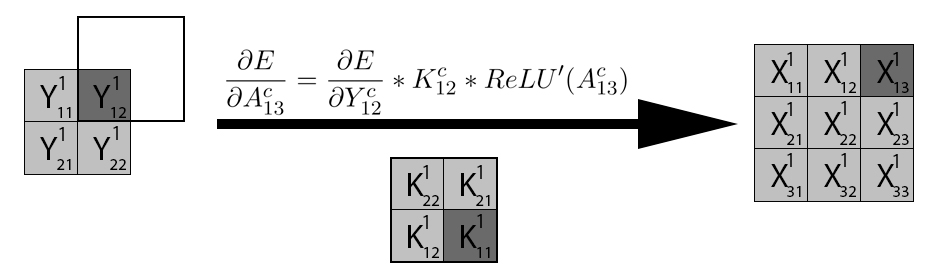
\includegraphics[width=1.4\linewidth]{imagenes/conv_back_entrada_3.jpg}  
		\caption{Gradiente con respecto a $X^1_{13}$}
	\end{subfigure}%
	\begin{subfigure}{.5\textwidth}
		\hspace{5mm}
		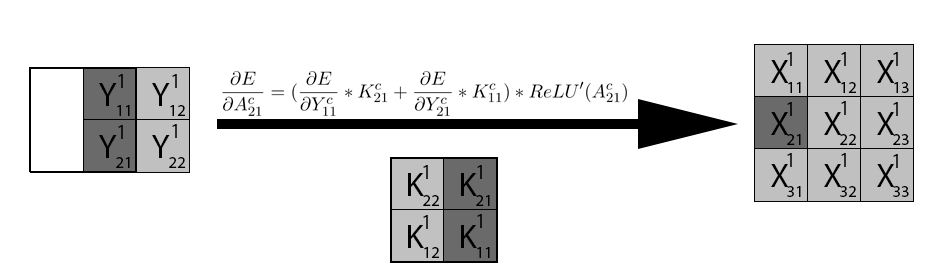
\includegraphics[width=1.4\linewidth]{imagenes/conv_back_entrada_4.jpg}  
		\caption{Gradiente con respecto a $X^1_{21}$}
	\end{subfigure}
	\vspace{5mm}
	\begin{subfigure}{.5\textwidth}
		\hspace{-25mm}
		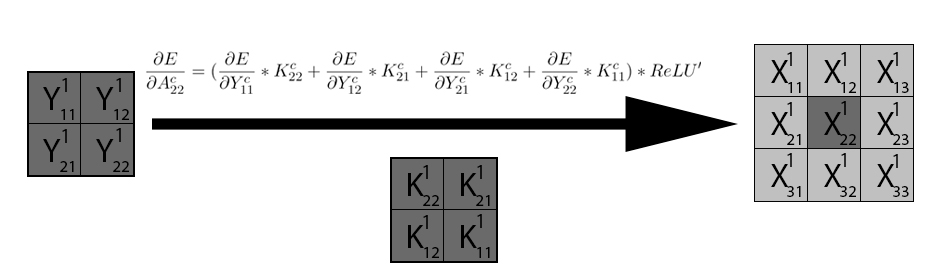
\includegraphics[width=1.4\linewidth]{imagenes/conv_back_entrada_5.jpg}  
		\caption{Gradiente con respecto a $X^1_{22}$}
	\end{subfigure}%
	\begin{subfigure}{.5\textwidth}
		\hspace{5mm}
		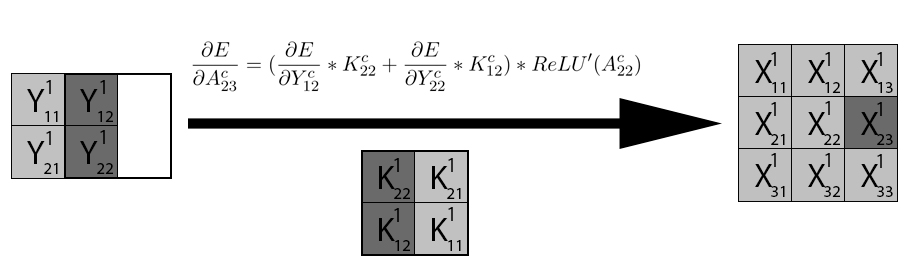
\includegraphics[width=1.4\linewidth]{imagenes/conv_back_entrada_6.jpg}  
		\caption{Gradiente con respecto a $X^1_{23}$}
	\end{subfigure}
	\vspace{5mm}
	\begin{subfigure}{.5\textwidth}
		\hspace{-25mm}
		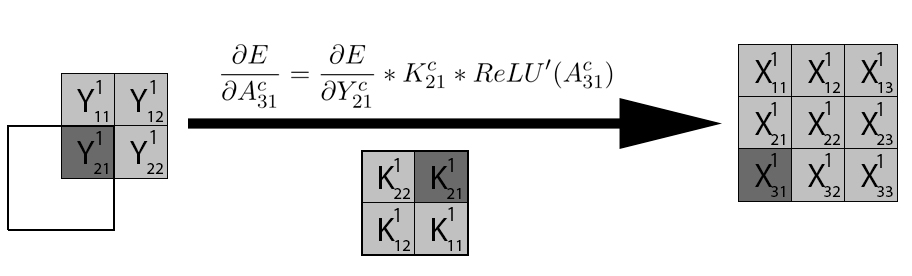
\includegraphics[width=1.4\linewidth]{imagenes/conv_back_entrada_7.jpg}  
		\caption{Gradiente con respecto a $X^1_{31}$}
	\end{subfigure}%
	\begin{subfigure}{.5\textwidth}
		\hspace{5mm}
		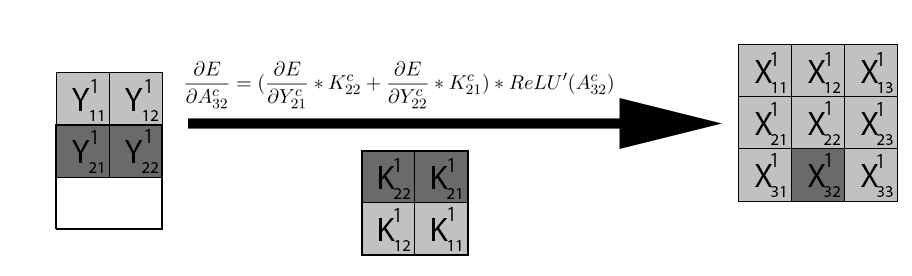
\includegraphics[width=1.4\linewidth]{imagenes/conv_back_entrada_8.jpg}  
		\caption{Gradiente con respecto a $X^1_{32}$}
	\end{subfigure}
	\vspace{5mm}
	\begin{subfigure}{.5\textwidth}
		\hspace{-25mm}
		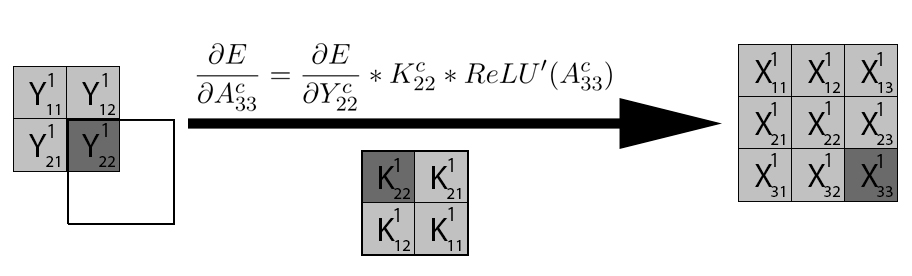
\includegraphics[width=1.4\linewidth]{imagenes/conv_back_entrada_9.jpg}  
		\caption{Gradiente con respecto a $X^1_{33}$}
	\end{subfigure}
	\caption{Cálculo del gradiente de la pérdida con respecto a cada valor de entrada como convolución entre K e Y}
	\label{fig:conv_backprop_como_convolucion_Y_W_apendice}
\end{figure}

Una vez más, los cálculos presentados en la Figura \ref{fig:conv_backprop_como_convolucion_Y_W} coinciden perfectamente con los obtenidos anteriormente, ya que son idénticos. La única diferencia radica en la manera de presentación, la cual ha sido adaptada para ofrecer una comprensión más y generalizada del proceso. Esta adaptación facilita la automatización de los cálculos y permite una implementación más eficiente en el código.

\section{Retropropagación con relleno}

\begin{figure}[H]
	\centering
	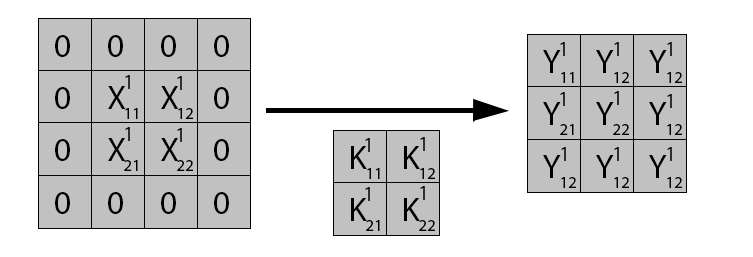
\includegraphics[width=0.8\linewidth]{imagenes/conv_back_padding_intro.jpg} 
	\caption{Ejemplo de retropropagación en una capa convolucional con relleno}
	\label{fig:conv_back_padding_intro}
\end{figure}

De manera similar al apartado anterior, se realizará y presentará el cálculo de la retropropagación para una capa convolucional. La diferencia principal en este caso radica en la inclusión de relleno en la capa, como se ilustra en el ejemplo proporcionado en la Figura \ref{fig:conv_back_padding_intro}. En consecuencia, se procederá a calcular el gradiente de la función de error con respecto a los pesos y a los valores de entrada de la capa.

\subsection{Gradiente de $Y^c_{11}$}

\begin{figure}[H]
	\centering
	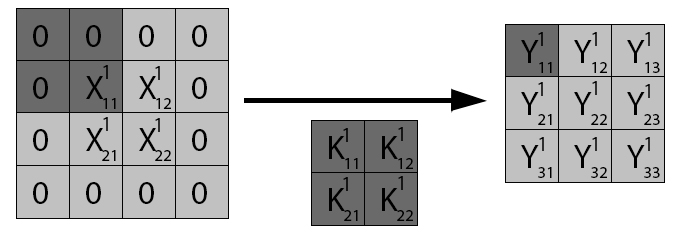
\includegraphics[width=0.8\linewidth]{imagenes/conv_back_padding_1.jpg} 
	\caption{Retropropagación de $Y^c_{11}$}
\end{figure}

Para facilitar la compresión del lector, se conservará la misma estructura y notación empleadas en el apartado anterior. Así, se procederá al cálculo del gradiente de $Y^c_{11}$ con respecto a cada peso utilizando las fórmulas \ref{gradr_Y11_w_1} y \ref{gradr_Y11_w_1}.

\begin{gather}
	Y^c_{11} = Z^c_{11}   K^c_{22} \\
	\frac{\partial Y^c_{11}}{\partial K^c_{xy}} = \frac{\partial (Z^c_{11}   K^c_{22})}{\partial K^c_{xy}} \\
	\frac{\partial Y^c_{11}}{\partial K^c_{11}} = 0, \hspace{10mm} \frac{\partial Y^c_{11}}{\partial K^c_{12}} = 0 \hspace{3mm} \label{gradr_Y11_w_1} \\
	\frac{\partial Y^c_{11}}{\partial K^c_{21}} = 0, \hspace{10mm} \frac{\partial Y^c_{11}}{\partial K^c_{22}} = Z^c_{11} \label{gradr_Y11_w_2}
\end{gather}

Para mantener la coherencia con el apartado anterior, también se calculará el gradiente de $Y^c_{11}$ con respecto a cada valor del volumen de entrada utilizando las fórmulas \ref{gradr_Y11_z_1} y \ref{gradr_Y11_z_2}.

\begin{gather}
	\frac{\partial Y^c_{11}}{\partial Z^c_{11}} = K^c_{22}, \hspace{10mm} \frac{\partial Y^c_{11}}{\partial Z^c_{12}} = 0 \label{gradr_Y11_z_1} \\
	\frac{\partial Y^c_{11}}{\partial Z^c_{21}} = 0, \hspace{14mm} \frac{\partial Y^c_{11}}{\partial Z^c_{22}} = 0 \label{gradr_Y11_z_2}
\end{gather}


\subsection{Gradiente de $Y^c_{12}$}

\begin{figure}[H]
	\centering
	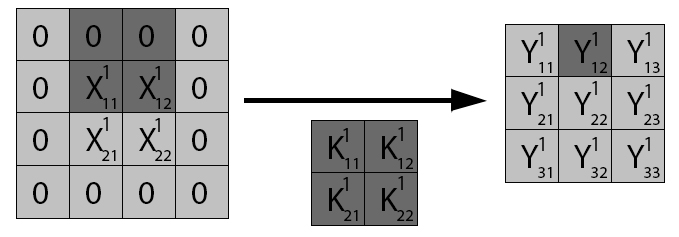
\includegraphics[width=0.8\linewidth]{imagenes/conv_back_padding_2.jpg} 
	\caption{Retropropagación de $Y^c_{12}$}
\end{figure}

Se calculará el gradiente de $Y^c_{12}$ con respecto a cada peso utilizando las fórmulas \ref{gradr_Y12_w_1} y \ref{gradr_Y12_w_2}.

\begin{gather}
	Y^c_{12} = Z^c_{11}   K^c_{21} + Z^c_{12}   K^c_{22} \\
	\frac{\partial Y^c_{12}}{\partial K^c_{xy}} = \frac{\partial (Z^c_{11}   K^c_{21} + Z^c_{12}   K^c_{22})}{\partial K^c_{xy}} \\
	\frac{\partial Y^c_{12}}{\partial K^c_{11}} = 0, \hspace{10mm} \frac{\partial Y^c_{12}}{\partial K^c_{12}} = 0 \label{gradr_Y12_w_1} \\
	\frac{\partial Y^c_{12}}{\partial K^c_{21}} = Z^c_{11}, \hspace{10mm} \frac{\partial Y^c_{12}}{\partial K^c_{22}} = Z^c_{12} \label{gradr_Y12_w_2}
\end{gather}

Asimismo, se calculará el gradiente de $Y^c_{12}$ con respecto a cada valor del volumen de entrada utilizando las fórmulas \ref{gradr_Y12_z_1} y \ref{gradr_Y12_z_2}.

\begin{gather}
	\frac{\partial Y^c_{12}}{\partial Z^c_{11}} = K^c_{21}, \hspace{10mm} \frac{\partial Y^c_{12}}{\partial Z^c_{12}} = K^c_{22} \label{gradr_Y12_z_1} \\
	\frac{\partial Y^c_{12}}{\partial Z^c_{21}} = 0, \hspace{14mm} \frac{\partial Y^c_{12}}{\partial Z^c_{22}} = 0 \hspace{4mm} \label{gradr_Y12_z_2}
\end{gather}

\subsection{Gradiente de $Y^c_{13}$}

\begin{figure}[H]
	\centering
	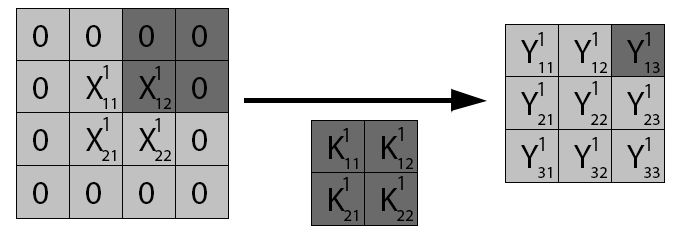
\includegraphics[width=0.8\linewidth]{imagenes/conv_back_padding_3.jpg} 
	\caption{Retropropagación de $Y^c_{13}$}
\end{figure}

Se calculará el gradiente de $Y^c_{13}$ con respecto a cada peso mediante las fórmulas \ref{gradr_Y13_w_1} y \ref{gradr_Y13_w_2}.

\begin{gather}
	Y^c_{13} = Z^c_{12}   K^c_{21} \\
	\frac{\partial Y^c_{13}}{\partial K^c_{xy}} = \frac{\partial (Z^c_{12}   K^c_{21})}{\partial K^c_{xy}} \\
	\frac{\partial Y^c_{13}}{\partial K^c_{11}} = 0, \hspace{13mm} \frac{\partial Y^c_{13}}{\partial K^c_{12}} = 0 \label{gradr_Y13_w_1} \\
	\frac{\partial Y^c_{13}}{\partial K^c_{21}} = Z^c_{12}, \hspace{10mm} \frac{\partial Y^c_{13}}{\partial K^c_{22}} = 0
\end{gather} \label{gradr_Y13_w_2}

Además, se calculará el gradiente de $Y^c_{13}$ con respecto a cada valor del volumen de entrada mediante las fórmulas \ref{gradr_Y13_z_1} y \ref{gradr_Y13_z_2}.

\begin{gather}
	\frac{\partial Y^c_{13}}{\partial Z^c_{11}} = 0, \hspace{10mm} \frac{\partial Y^c_{13}}{\partial Z^c_{12}} = K^c_{21} \label{gradr_Y13_z_1} \\
	\frac{\partial Y^c_{13}}{\partial Z^c_{21}} = 0, \hspace{14mm} \frac{\partial Y^c_{13}}{\partial Z^c_{22}} = 0 \hspace{4mm} \label{gradr_Y13_z_2}
\end{gather}


\subsection{Gradiente de $Y^c_{21}$}

\begin{figure}[H]
	\centering
	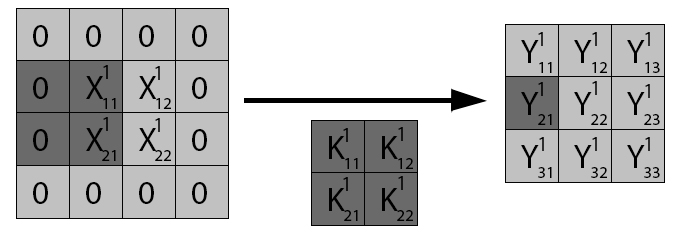
\includegraphics[width=0.8\linewidth]{imagenes/conv_back_padding_4.jpg} 
	\caption{Retropropagación de $Y^c_{21}$}
\end{figure}

Se calculará el gradiente de $Y^c_{21}$ con respecto a cada peso utilizando las fórmulas \ref{gradr_Y21_w_1} y \ref{gradr_Y21_w_2}.


\begin{gather}
	Y^c_{21} = Z^c_{11}   K^c_{12} + Z^c_{21}   K^c_{22} \\
	\frac{\partial Y^c_{21}}{\partial K^c_{xy}} = \frac{\partial (Z^c_{11}   K^c_{12} + Z^c_{21}   K^c_{22})}{\partial K^c_{xy}} \\
	\frac{\partial Y^c_{21}}{\partial K^c_{11}} = 0, \hspace{10mm} \frac{\partial Y^c_{21}}{\partial K^c_{12}} = Z^c_{11} \label{gradr_Y21_w_1} \\
	\frac{\partial Y^c_{21}}{\partial K^c_{21}} = 0, \hspace{10mm} \frac{\partial Y^c_{21}}{\partial K^c_{22}} = Z^c_{21} \label{gradr_Y21_w_2}
\end{gather}

Además, se calculará el gradiente de $Y^c_{21}$ con respecto a cada valor del volumen de entrada utilizando las fórmulas \ref{gradr_Y21_z_1} y \ref{gradr_Y21_z_2}.

\begin{gather}
	\frac{\partial Y^c_{21}}{\partial Z^c_{11}} = K^c_{12}, \hspace{10mm} \frac{\partial Y^c_{21}}{\partial Z^c_{12}} = 0 \label{gradr_Y21_z_1} \\
	\frac{\partial Y^c_{21}}{\partial Z^c_{21}} = K^c_{22}, \hspace{10mm} \frac{\partial Y^c_{21}}{\partial Z^c_{22}} = 0
\end{gather} \label{gradr_Y21_z_2}

\subsection{Gradiente de $Y^c_{22}$}

\begin{figure}[H]
	\centering
	\includegraphics[width=0.8\linewidth]{imagenes/conv_back_padding_5.jpg} 
	\caption{Retropropagación de $Y^c_{22}$}
\end{figure}

Se calculará el gradiente de $Y^c_{22}$ con respecto a cada peso utilizando las fórmulas \ref{gradr_Y22_w_1} y \ref{gradr_Y22_w_2}.


\begin{gather}
	Y^c_{22} = Z^c_{11}   K^c_{11} + Z^c_{12}   K^c_{12} + Z^c_{21}   K^c_{21} + Z^c_{22}   K^c_{22} \\
	\frac{\partial Y^c_{22}}{\partial K^c_{xy}} = \frac{\partial (Z^c_{11}   K^c_{11} + Z^c_{12}   K^c_{12} + Z^c_{21}   K^c_{21} + Z^c_{22}   K^c_{22})}{\partial K^c_{xy}} \\
	\frac{\partial Y^c_{22}}{\partial K^c_{11}} = Z^c_{11}, \hspace{10mm} \frac{\partial Y^c_{22}}{\partial K^c_{12}} = Z^c_{12} \label{gradr_Y22_w_1} \\
	\frac{\partial Y^c_{22}}{\partial K^c_{21}} = Z^c_{21}, \hspace{10mm} \frac{\partial Y^c_{22}}{\partial K^c_{22}} = Z^c_{22} \label{gradr_Y22_w_2}
\end{gather}

Asimismo, se calculará el gradiente de $Y^c_{22}$ con respecto a cada valor del volumen de entrada mediante las fórmulas \ref{gradr_Y22_z_1} y \ref{gradr_Y22_z_2}.

\begin{gather}
	\frac{\partial Y^c_{22}}{\partial Z^c_{11}} = K^c_{11}, \hspace{10mm} \frac{\partial Y^c_{22}}{\partial Z^c_{12}} = K^c_{12} \label{gradr_Y22_z_1} \\
	\frac{\partial Y^c_{22}}{\partial Z^c_{21}} = K^c_{21}, \hspace{10mm} \frac{\partial Y^c_{22}}{\partial Z^c_{22}} = K^c_{22} \label{gradr_Y22_z_2}.
\end{gather}

\subsection{Gradiente de $Y^c_{23}$}

\begin{figure}[H]
	\centering
	\includegraphics[width=0.8\linewidth]{imagenes/conv_back_padding_6.jpg} 
	\caption{Retropropagación de $Y^c_{23}$}
\end{figure}

Se calculará el gradiente de $Y^c_{23}$ con respecto a cada peso utilizando las fórmulas \ref{gradr_Y23_w_1} y \ref{gradr_Y23_w_2}.


\begin{gather}
	Y^c_{23} = Z^c_{12}   K^c_{11} + Z^c_{22}   K^c_{21} \\
	\frac{\partial Y^c_{23}}{\partial K^c_{xy}} = \frac{\partial (Z^c_{12}   K^c_{11} + Z^c_{22}   K^c_{21})}{\partial K^c_{xy}} \\
	\frac{\partial Y^c_{23}}{\partial K^c_{11}} = Z^c_{12}, \hspace{10mm} \frac{\partial Y^c_{23}}{\partial K^c_{12}} = 0 \label{gradr_Y23_w_1} \\
	\frac{\partial Y^c_{23}}{\partial K^c_{21}} = Z^c_{22}, \hspace{10mm} \frac{\partial Y^c_{23}}{\partial K^c_{22}} = 0 \label{gradr_Y23_w_2}
\end{gather}

De igual manera, se calculará el gradiente de $Y^c_{23}$ con respecto a cada valor del volumen de entrada mediante las fórmulas \ref{gradr_Y22_z_1} y \ref{gradr_Y22_z_2}.


\begin{gather}
	\frac{\partial Y^c_{23}}{\partial Z^c_{11}} = 0, \hspace{10mm} \frac{\partial Y^c_{23}}{\partial Z^c_{12}} = K^c_{11}\\
	\frac{\partial Y^c_{23}}{\partial Z^c_{21}} = 0, \hspace{10mm} \frac{\partial Y^c_{23}}{\partial Z^c_{22}} = K^c_{21}
\end{gather}

\subsection{Gradiente de $Y^c_{31}$}

\begin{figure}[H]
	\centering
	\includegraphics[width=0.8\linewidth]{imagenes/conv_back_padding_7.jpg} 
	\caption{Retropropagación de $Y^c_{31}$}
\end{figure}

Se calculará el gradiente de $Y^c_{31}$ con respecto a cada peso utilizando las fórmulas \ref{gradr_Y31_w_1} y \ref{gradr_Y31_w_2}.

\begin{gather}
	Y^c_{31} = Z^c_{21}   K^c_{12} \\
	\frac{\partial Y^c_{31}}{\partial K^c_{xy}} = \frac{\partial (Z^c_{21}   K^c_{12})}{\partial K^c_{xy}} \\
	\frac{\partial Y^c_{31}}{\partial K^c_{11}} = 0, \hspace{10mm} \frac{\partial Y^c_{31}}{\partial K^c_{12}} = Z^c_{21} \label{gradr_Y31_w_1} \\
	\frac{\partial Y^c_{31}}{\partial K^c_{21}} = 0, \hspace{10mm} \frac{\partial Y^c_{31}}{\partial K^c_{22}} = 0 \hspace{4mm} \label{gradr_Y31_w_2}
\end{gather}

Asimismo, se calculará el gradiente de $Y^c_{31}$ con respecto a cada valor del volumen de entrada mediante las fórmulas \ref{gradr_Y31_z_1} y \ref{gradr_Y31_z_2}.

\begin{gather}
	\frac{\partial Y^c_{31}}{\partial Z^c_{11}} = 0, \hspace{14mm} \frac{\partial Y^c_{31}}{\partial Z^c_{12}} = 0 \label{gradr_Y31_z_1} \\
	\frac{\partial Y^c_{31}}{\partial Z^c_{21}} = K^c_{12}, \hspace{10mm} \frac{\partial Y^c_{31}}{\partial Z^c_{22}} = 0 \label{gradr_Y31_z_2}
\end{gather}


\subsection{Gradiente de $Y^c_{32}$}

\begin{figure}[H]
	\centering
	\includegraphics[width=0.8\linewidth]{imagenes/conv_back_padding_8.jpg} 
	\caption{Retropropagación de $Y^c_{32}$}
\end{figure}

Se calculará el gradiente de $Y^c_{32}$ con respecto a cada peso utilizando las fórmulas \ref{gradr_Y32_w_1} y \ref{gradr_Y32_w_2}.

\begin{gather}
	Y^c_{32} = Z^c_{21}   K^c_{11} + Z^c_{22}   K^c_{12} \\
	\frac{\partial Y^c_{32}}{\partial K^c_{xy}} = \frac{\partial (Z^c_{21}   K^c_{11} + Z^c_{22}   K^c_{12})}{\partial K^c_{xy}} \\
	\frac{\partial Y^c_{32}}{\partial K^c_{11}} = Z^c_{21}, \hspace{10mm} \frac{\partial Y^c_{32}}{\partial K^c_{12}} = Z^c_{22} \label{gradr_Y32_w_1} \\
	\frac{\partial Y^c_{32}}{\partial K^c_{21}} = 0, \hspace{14mm} \frac{\partial Y^c_{32}}{\partial K^c_{22}} = 0 \hspace{4mm} \label{gradr_Y32_w_2}
\end{gather}

Además, se calculará el gradiente de $Y^c_{32}$ con respecto a cada valor del volumen de entrada mediante las fórmulas \ref{gradr_Y32_z_1} y \ref{gradr_Y32_z_2}.


\begin{gather}
	\frac{\partial Y^c_{32}}{\partial Z^c_{11}} = 0, \hspace{14mm} \frac{\partial Y^c_{32}}{\partial Z^c_{12}} = 0 \hspace{4mm} \label{gradr_Y32_z_1} \\
	\frac{\partial Y^c_{32}}{\partial Z^c_{21}} = K^c_{11}, \hspace{10mm} \frac{\partial Y^c_{32}}{\partial Z^c_{22}} = K^c_{12} \label{gradr_Y32_z_2}
\end{gather}



\subsection{Gradiente de $Y^c_{33}$}

\begin{figure}[H]
	\centering
	\includegraphics[width=0.8\linewidth]{imagenes/conv_back_padding_9.jpg} 
	\caption{Retropropagación de $Y^c_{33}$}
\end{figure}

Se calculará el gradiente de $Y^c_{33}$ con respecto a cada peso utilizando las fórmulas \ref{gradr_Y33_w_1} y \ref{gradr_Y33_w_2}.


\begin{gather}
	Y^c_{33} = Z^c_{22}   K^c_{11} \\
	\frac{\partial Y^c_{33}}{\partial K^c_{xy}} = \frac{\partial (Z^c_{22}   K^c_{11})}{\partial K^c_{xy}} \\
	\frac{\partial Y^c_{33}}{\partial K^c_{11}} = Z^c_{22}, \hspace{10mm} \frac{\partial Y^c_{33}}{\partial K^c_{12}} = 0 \label{gradr_Y33_w_1} \\
	\frac{\partial Y^c_{33}}{\partial K^c_{21}} = 0, \hspace{14mm} \frac{\partial Y^c_{33}}{\partial K^c_{22}} = 0 \label{gradr_Y33_w_2}
\end{gather}

Asimismo, se calculará el gradiente de $Y^c_{33}$ con respecto a cada valor del volumen de entrada utilizando las fórmulas \ref{gradr_Y33_z_1} y \ref{gradr_Y33_z_2}.


\begin{gather}
	\frac{\partial Y^c_{33}}{\partial Z^c_{11}} = 0, \hspace{10mm} \frac{\partial Y^c_{33}}{\partial Z^c_{12}} = 0 \hspace{4mm} \label{gradr_Y33_z_1} \\
	\frac{\partial Y^c_{33}}{\partial Z^c_{21}} = 0, \hspace{10mm} \frac{\partial Y^c_{33}}{\partial Z^c_{22}} = K^c_{11} \label{gradr_Y33_z_2}
\end{gather}


\subsection{Gradiente respecto a pesos como convolución}

Finalmente, de manera similar al caso anterior, se calcula la sumatoria de los gradientes y, con ello, el gradiente de la función de pérdida con respecto a cada peso $K_{xy}$. Nuevamente, se identifica un patrón claro en los resultados obtenidos.

\begin{gather}
	\frac{\partial E}{\partial K^c_{11}} = \frac{\partial E}{\partial Y^c_{22}}   Z^c_{11} + \frac{\partial E}{\partial Y^c_{23}}   Z^c_{12} + \frac{\partial E}{\partial Y^c_{32}}   Z^c_{21} + \frac{\partial E}{\partial Y^c_{33}}   Z^c_{22} \label{result_conv_1_apendice} \\
	\frac{\partial E}{\partial K^c_{12}} = \frac{\partial E}{\partial Y^c_{21}}   Z^c_{11} + \frac{\partial E}{\partial Y^c_{22}}   Z^c_{12} + \frac{\partial E}{\partial Y^c_{31}}   Z^c_{21} + \frac{\partial E}{\partial Y^c_{32}}   Z^c_{22} \label{result_conv_2_apendice} \\
	\frac{\partial E}{\partial K^c_{21}} = \frac{\partial E}{\partial Y^c_{12}}   Z^c_{11} + \frac{\partial E}{\partial Y^c_{13}}   Z^c_{12} + \frac{\partial E}{\partial Y^c_{22}}   Z^c_{21} + \frac{\partial E}{\partial Y^c_{23}}   Z^c_{22} \label{result_conv_3_apendice} \\
	\frac{\partial E}{\partial K^c_{22}} = \frac{\partial E}{\partial Y^c_{11}}   Z^c_{11} + \frac{\partial E}{\partial Y^c_{12}}   Z^c_{12} + \frac{\partial E}{\partial Y^c_{21}}   Z^c_{21} + \frac{\partial E}{\partial Y^c_{22}}   Z^c_{22} \label{result_conv_4_apendice}
\end{gather}

Como se puede observar en los cálculos obtenidos (véanse las fórmulas \ref{result_conv_1_apendice}, \ref{result_conv_2_apendice}, \ref{result_conv_3_apendice}, y \ref{result_conv_4_apendice}), estos coinciden con una convolución entre la entrada X con relleno, y el gradiente con respecto a la capa de salida Y, como se ilustra en la Figura \ref{fig:conv_backprop_como_convolucion_Xpad_Y}. Como era de esperar, los resultados son equivalentes a los obtenidos ene el caso anterior, con la única diferencia de que ahora se emplea X con relleno en lugar de X sin relleno para realizar la convolución.

\begin{figure}[H]
	\centering
	\begin{subfigure}{.5\textwidth}
		\hspace{-25mm}
		\includegraphics[width=1.4\linewidth]{imagenes/conv_back_pad_1.jpg}  
		\caption{Cálculo de $\frac{\partial E}{\partial K^1_{11}}$}
	\end{subfigure}%
	\begin{subfigure}{.5\textwidth}
		\hspace{5mm}
		\includegraphics[width=1.4\linewidth]{imagenes/conv_back_pad_2.jpg}  
		\caption{Cálculo de $\frac{\partial E}{\partial K^1_{12}}$}
	\end{subfigure}
	\vspace{5mm}
	\begin{subfigure}{.5\textwidth}
		\hspace{-25mm}
		\includegraphics[width=1.4\linewidth]{imagenes/conv_back_pad_3.jpg}  
		\caption{Cálculo de $\frac{\partial E}{\partial K^1_{21}}$}
	\end{subfigure}%
	\begin{subfigure}{.5\textwidth}
		\hspace{5mm}
		\includegraphics[width=1.4\linewidth]{imagenes/conv_back_pad_4.jpg}  
		\caption{Cálculo de $\frac{\partial E}{\partial K^1_{22}}$}
	\end{subfigure}
	\caption{Cálculo del gradiente de la pérdida con respecto a cada filtro como convolución entre X e Y}
	\label{fig:conv_backprop_como_convolucion_Xpad_Y}
\end{figure}

\subsection{Gradiente respecto a entrada como convolución}

Una vez más, se utilizará la función de activación ReLU en las capas convolucionales, conforme a lo discutido anteriormente. Por consiguiente, la derivada de esta función ya ha sido determinada previamente (véase la fórmula \ref{deriv_relu}).


\begin{gather}
	\frac{\partial E}{\partial A^c_{11}} = (\frac{\partial E}{\partial Y^c_{11}}   K^c_{22} + \frac{\partial E}{\partial Y^c_{12}}   K^c_{21} + \frac{\partial E}{\partial Y^c_{21}}   K^c_{12} + \frac{\partial E}{\partial Y^c_{22}}   K^c_{11})    ReLU'(A^c_{11}) \label{result_conv_x1} \\
	\frac{\partial E}{\partial A^c_{12}} = (\frac{\partial E}{\partial Y^c_{12}}   K^c_{22} + \frac{\partial E}{\partial Y^c_{13}}   K^c_{21} + \frac{\partial E}{\partial Y^c_{22}}   K^c_{12} + \frac{\partial E}{\partial Y^c_{23}}   K^c_{11})   ReLU'(A^c_{21}) \label{result_conv_x2} \\
	\frac{\partial E}{\partial A^c_{21}} = (\frac{\partial E}{\partial Y^c_{21}}   K^c_{22} + \frac{\partial E}{\partial Y^c_{22}}   K^c_{21} + \frac{\partial E}{\partial Y^c_{31}}   K^c_{12} + \frac{\partial E}{\partial Y^c_{32}}   K^c_{11})   ReLU'(A^c_{21}) \label{result_conv_x3} \\
	\frac{\partial E}{\partial A^c_{22}} = (\frac{\partial E}{\partial Y^c_{22}}   K^c_{22} + \frac{\partial E}{\partial Y^c_{23}}   K^c_{21} + \frac{\partial E}{\partial Y^c_{32}}   K^c_{12} + \frac{\partial E}{\partial Y^c_{33}}   K^c_{11})   ReLU'(A^c_{22}) \label{result_conv_x4}
\end{gather}

Como se observa en los cálculos obtenidos (véanse las fórmulas \ref{result_conv_x1}, \ref{result_conv_x2}, \ref{result_conv_x3}, y \ref{result_conv_x4}), los resultados coinciden con una convolución entre el gradiente con respecto a la capa de salida Y y los pesos K, invertidos tanto horizontal como verticalmente. Este proceso se ilustra en detalle en la figura \ref{fig:conv_backprop_como_convolucion_Y_K_pad}.

\begin{figure}[H]
	\centering
	\begin{subfigure}{.5\textwidth}
		\hspace{-25mm}
		\includegraphics[width=1.4\linewidth]{imagenes/conv_back_entrada_pad_1.jpg}  
		\caption{Cálculo de $\frac{\partial E}{\partial A^1_{11}}$}
	\end{subfigure}%
	\begin{subfigure}{.5\textwidth}
		\hspace{5mm}
		\includegraphics[width=1.4\linewidth]{imagenes/conv_back_entrada_pad_2.jpg}  
		\caption{Cálculo de $\frac{\partial E}{\partial A^1_{12}}$}
	\end{subfigure}
	\vspace{5mm}
	\begin{subfigure}{.5\textwidth}
		\hspace{-25mm}
		\includegraphics[width=1.4\linewidth]{imagenes/conv_back_entrada_pad_3.jpg}  
		\caption{Cálculo de $\frac{\partial E}{\partial A^1_{21}}$}
	\end{subfigure}%
	\begin{subfigure}{.5\textwidth}
		\hspace{5mm}
		\includegraphics[width=1.4\linewidth]{imagenes/conv_back_entrada_pad_4.jpg}  
		\caption{Cálculo de $\frac{\partial E}{\partial A^1_{22}}$}
	\end{subfigure}
	\caption{Cálculo del gradiente de la pérdida con respecto a la entrada como convolución}
	\label{fig:conv_backprop_como_convolucion_Y_K_pad}
\end{figure}

Una vez desarrolladas ambas retropropagaciones en una capa convolucional, tanto con relleno como sin relleno, se pueden comparar las figuras \ref{fig:conv_backprop_como_convolucion_Y_W_apendice} y \ref{fig:conv_backprop_como_convolucion_Y_K_pad}. Em ambas representaciones, se calcula el gradiente de la pérdida con respecto al volumen de entrada. No obstante, se observa que en la primera figura se utiliza una convolución con relleno completo sobre el volumen Y (volumen de salida de la capa), mientras que en la segunda figura se aplica una convolución sin relleno.


\begin{figure}[H]
	\centering
	\begin{subfigure}{.5\textwidth}
		\includegraphics[width=1.4\linewidth]{imagenes/full_vs_normal_conv_1.jpg}  
		\caption{Retropropagación con un nivel de relleno}
	\end{subfigure}
	
	\vspace{5mm}
	\begin{subfigure}{.5\textwidth}
		\includegraphics[width=1.4\linewidth]{imagenes/full_vs_normal_conv_2.jpg}  
		\caption{Retropropagación con dos niveles de relleno}
	\end{subfigure}
	\caption{Cálculo del gradiente de la pérdida con respecto a la entrada X con uno y dos niveles de relleno}
	\label{fig:conv_full_vs_normal_apendice}
\end{figure}

La razón detrás de esta diferencia se detalla en la figura \ref{fig:conv_full_vs_normal_apendice}. En el caso de una convolución con relleno completo, los gradientes se calculan comenzando desde la esquina superior izquierda de X. Sin embargo, dado que X incluye relleno, no es necesario calcular los gradientes en las posiciones de relleno, ya que estos valores no influyen en los cálculos posteriores.

%\input{capitulos/01\_Introduccion}
%
%\input{capitulos/02_EspecificacionRequisitos}
%
%\input{capitulos/03_Planificacion}
%
%\input{capitulos/04_Analisis}
%
%\input{capitulos/05_Diseno}
%
%\input{capitulos/06_Implementacion}
%
%\input{capitulos/07_Pruebas}
%
%\input{capitulos/08_Conclusiones}
%
%%\chapter{Conclusiones y Trabajos Futuros}
%
%
%%\nocite{*}
%\bibliography{bibliografia/bibliografia}\addcontentsline{toc}{chapter}{Bibliografía}
%\bibliographystyle{miunsrturl}
\bibliographystyle{unsrt}
\bibliography{bibliografia/bibliografia}


%
%\appendix
%\input{apendices/manual_usuario/manual_usuario}
%%\input{apendices/paper/paper}
%\input{glosario/entradas_glosario}
% \addcontentsline{toc}{chapter}{Glosario}
% \printglossary
\chapter*{}
\thispagestyle{empty}

\end{document}
